\section{Time Rectification and Accuracy}
\label{sec-timing}

%  - FTSP stability: How often did FTSP go down and for how long? [GWA]
%  - % of events with 'good' FTSP timing  [GWA]
%  - Accuracy of time rectification on Teloslab [GWA]
%    - Vary time rectification parameters

%\begin{figure}[t]
%\begin{center}
%\includegraphics[width=\hsize]{./casestudy/figs/timing/}
%\end{center}
%\caption{\small{\bf Title}
%{\em Description}}
%\label{fig-}
%\end{figure}

When analyzing seismoacoustic data acquired at volcanoes, accurate 
timing of recorded signals is paramount. Studying volcanic source processes
necessitates precisely identifying the arrival time of P-~and S-waves 
at each sensor. Also, correlating signals across the sensor
array requires accurately timestamping each sample.  Ideally, timing should
be accurate to within one sample interval, or 10~ms when sampling at 100~Hz.
% MDW 26-Aug-06: I think it's OK to not repeat the power-hungry nature
% of GPS receivers; we've said it a few times already.
As described earlier, 
%seismologists typically deploy a GPS receiver at each
%station. Because GPS receivers are expensive and power hungry, 
we opted to
use a single GPS receiver and employ a multihop time-synchronization protocol
to establish a global timebase. The protocol worked well
in laboratory experiments. However, it experienced significant failures in
the field, requiring extensive postprocessing of the data to recover accurate
timing for each signal.

In this section, we provide an overview of the time synchronization errors
observed in the field. We then present a novel {\em time rectification}
technique that allows us to recover accurate timing despite protocol
failures.  
%Prior internet measurement work has examined similar techniques
%for error detection and recovery and produced valuable insights and
%  advice~\cite{paxson98calibrating,1028824}
%However, the specific techniques do not map directly to our application for
%several reasons. First, they focus more on error detection and do not
%address rectification.  Second, the sensor network time synchronization
%protocols we deployed are new and have goals distinct from common network
%time-synchronization protocols. Additionally, most network measurements can
%be performed using relative times only, whereas the scientific requirements
%of our application required assigning an accurate absolute timestamp to
%each collected sample.
We evaluate our approach through
lab experiments with a known, ground-truth timebase, and by comparing our
signals with signals recorded by the colocated data loggers. This
paper is the first to our knowledge to evaluate the stability of a multihop
time synchronization protocol during a lengthy sensor network 
field deployment. 

\subsection{Time synchronization architecture}

We chose to use the Flooding Time Synchronization Protocol
(FTSP)~\cite{ftsp}, an existing protocol developed for
wireless sensor nodes.  In the original FTSP work~\cite{ftsp}, timing errors
of less than 67~$\mu$sec were reported for an 11-hop network of Mica2 nodes.
We verified in our testbed that FTSP provided a 90th-percentile time
error of under 2.1~ms in a 5-hop linear network of TMote Sky nodes.

A single MicaZ sensor node was used as the root of the FTSP synchronization
tree. It interfaced to a Garmin GPS receiver and received a 1~Hz interrupt
synchronized to within 1~$\mu$sec of the GPS ``pulse per second'' signal.
When the interrupt is raised, the node records the GPS time and corresponding
FTSP global time and sends a short message containing this information to the
base station.  Each sensor node runs the FTSP protocol which maintains a
global timebase. Every 10~sec, each node records its local time and the
corresponding FTSP global time, sending this information in its status
message to the base station. Finally, as each node records data, the first
sample of each block is marked with the node's local time. After downloading
data from each node following an event, this local time can be used to
recover the time for each sample in the block.

Therefore, we have three relevant timebases: the {\em local time} at each
node; the {\em global time} established by the FTSP protocol; and the
{\em GPS time} recorded by the FTSP root. The information in the nodes'
status messages can be used to map local time to global time, and the
information in the GPS node's status messages can be used to map global time
to GPS-based GMT.

\subsection{FTSP failures in the field}
\label{timing-deploymentfailures}

In the absence of failures, this mapping would be a straightforward process.
However, in the field, we noticed that nodes would occasionally lose
synchronization with the rest of the network and report FTSP global times
with significant errors, sometimes exceeding several hours. We suspect that
the sparse deployment conditions at the volcano might have led to different
behavior in the time synchronization protocol than in the lab. For
example, occasional message loss or failure of a neighbor could cause the 
node's global time to drift from the rest of the network.  
However, in lab tests that constrained the network topology we 
did not observe these instabilities.

\begin{figure}[t]
\begin{center}
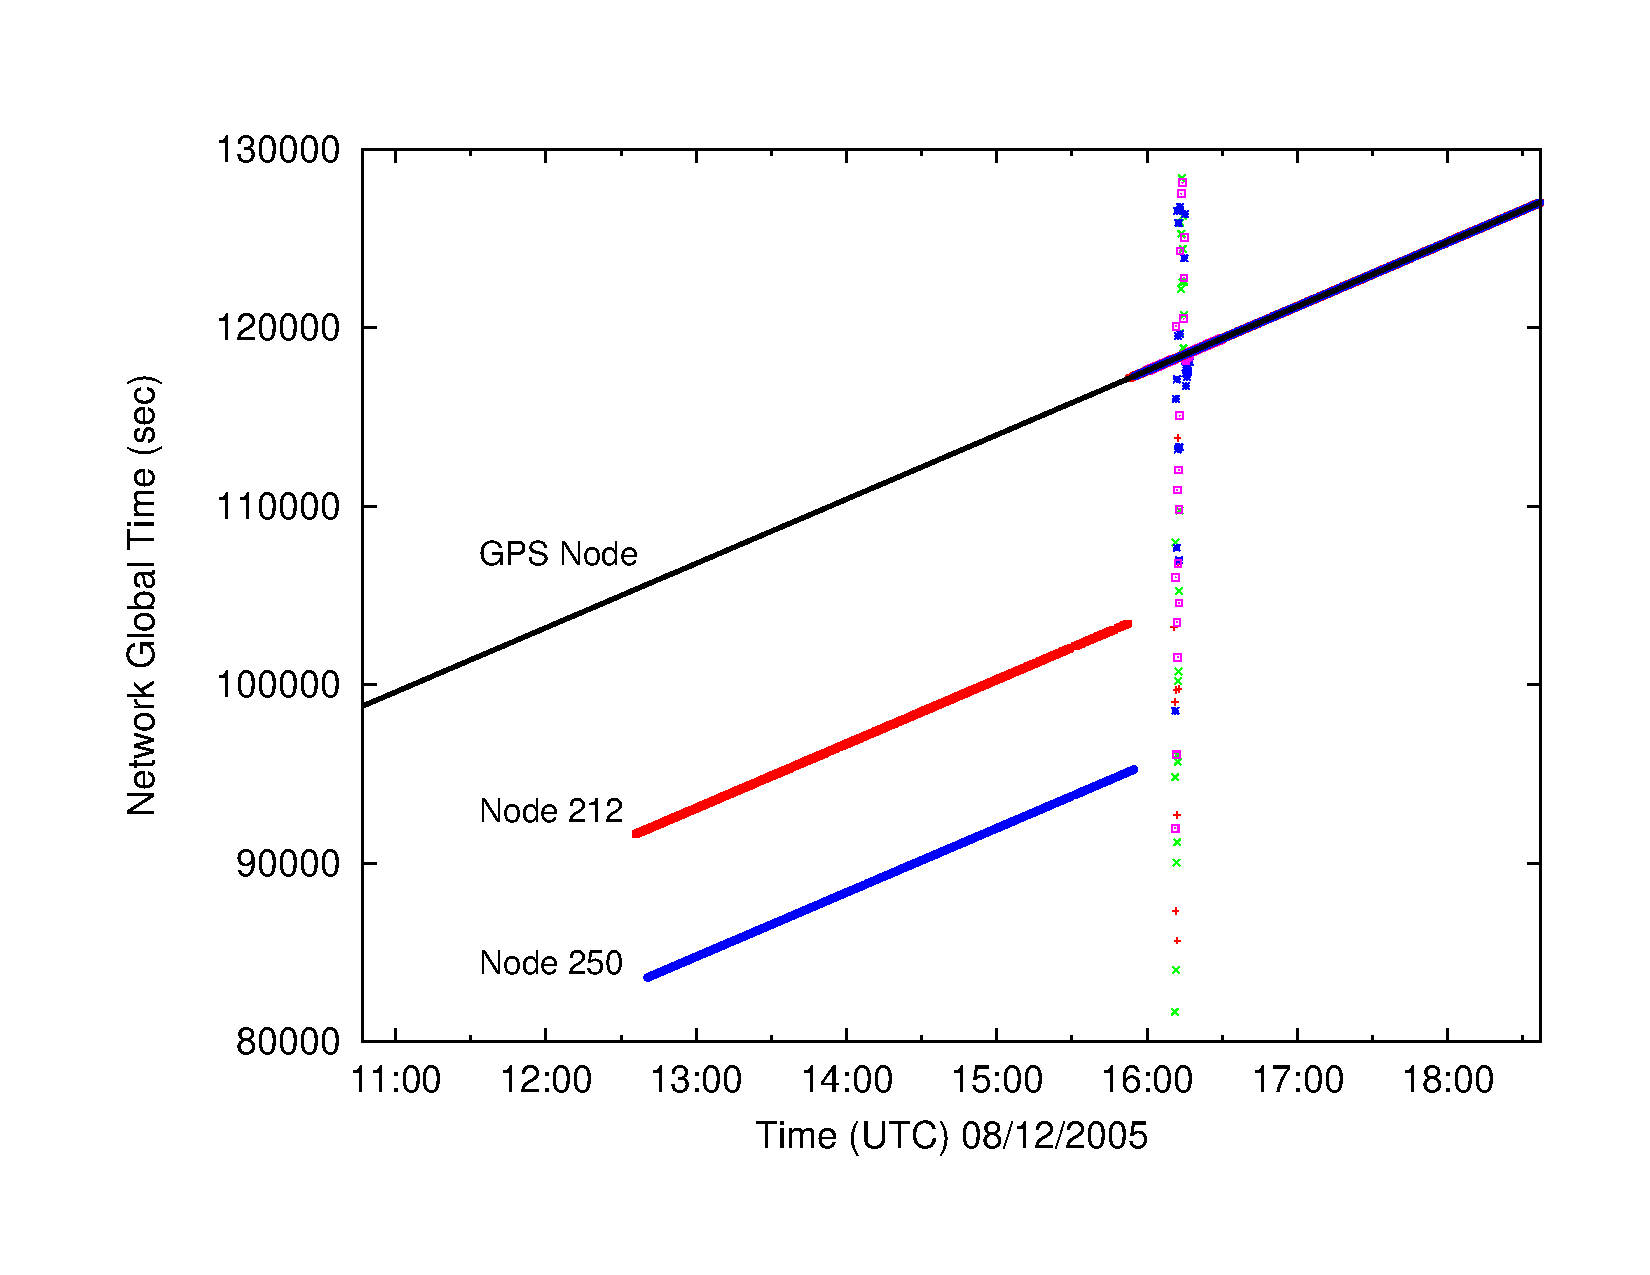
\includegraphics[width=\hsize]{./casestudy/figs/timing/MDW/instability/FTSPINSTABILITY.pdf}
\end{center} 

\caption{{\small {\bf Example of FTSP instability observed during field
deployment:} {\em The global time value reported by sensor nodes and the
GPS node is plotted against the time that the base station received the
corresponding status messages. All nodes are initially synchronized, but
starting at 1230 GMT, nodes 212~and~250 report incorrect global times for the
next 4.5~hours. When the nodes eventually resynchronize, the global
timestamps of other nodes initially experience some instability.}}}
\label{fig-globaltimeproblem}
\end{figure}

Figure~\ref{fig-globaltimeproblem} shows an example of the FTSP instability
observed in the field. The global time reported by two nodes
suddenly jumps off by several hours, and the nodes do not resynchronize until
rebooted 4.5~hours later.  It turns out that two bugs conflated to cause this
problem.  First, it was discovered that the TinyOS clock driver would
occasionally return bogus local timestamps.  This bug was fixed in
February 2006, several months after our deployment. 
Second, FTSP does not check the
validity of synchronization messages, so a node reading an incorrect 
value for its local clock can corrupt the state of other nodes, 
throwing off the global time calculation.  
To our knowledge, few if any sensor network deployments have
attempted to use network time synchronization protocols for extended periods.
In addition, ours may have been the first deployment of FTSP on the TMote Sky
platform where the clock driver bug manifested itself. 

\begin{figure}[t]
\begin{center}
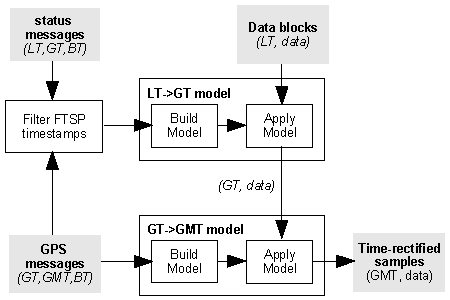
\includegraphics[width=0.8\hsize]{./casestudy/figs/timing/RectificationCartoon/cartoon.pdf}
\end{center}
\caption{\small{\bf Time rectification process overview.}}
\label{fig-rectificationcartoon}
\end{figure}

The failures of the time synchronization protocol make establishing the
correct GPS-based timestamp for each data sample extremely challenging. Our
{\em time rectification} approach filters and remaps recorded timestamps to
accurately recover timing despite these failures.  The time rectification
process is illustrated in Figure~\ref{fig-rectificationcartoon}. The first
step is to {\em filter} the global timestamps recorded by each node,
discarding bogus data. Second, we build a model mapping the local time on
each node to FTSP-based global time.  Third, we use the GPS timestamp
information to build a second model mapping FTSP time to GMT. Finally, both
models are applied to the timestamps recorded in each data block producing a
GMT time for each sample.

\subsection{Timestamp filtering}
\label{subsection-filtering}

We begin by filtering out status messages appearing to contain incorrect
global timestamps. To do this, we correlate global timestamps from each node
against a common reference timebase and reject those that differ by more than
some threshold.  For this, we use the base station laptop's local time, which
is {\em only} used for filtering FTSP timestamps, not for establishing the
correct timing. The filtering process in is many ways similar to prior
work~\cite{paxson98calibrating,1028824} on detecting adjustments in
network-synchronized clocks. % when analyzing network packet traces.

We use the following abbreviations: {\em LT} is the local
time of a node; {\em GT} is the FTSP global time; {\em BT} is the base
station's local time; and {\em GMT} is the true GMT from the GPS signal.
Each GPS status message logged by the base station consists of the 
triple {\em (GT, GMT, BT)}. 
We use linear regression on this data to produce a reference
timebase mapping {\em BT} to {\em GT}.\footnote{We assume that the global
time reported by the GPS node is always correct; indeed, the definition of
``global time'' is the FTSP time reported by the GPS node. We verified that
the FTSP instability affecting the sensor nodes did not occur on the GPS
node, most likely because the MicaZ uses a different processor that is
unaffected by the clock driver bug.} For each node status message logged by
the laptop {\em (LT, GT, BT)}, we map {\em BT} to the expected
$\mathit{GT}_{\mathit{ref}}$ using the reference timebase. If $ \mid
\mathit{GT}_{\mathit{ref}} - \mathit{GT} \mid > \delta$, we discard the
status message from further consideration.  We use a threshold of $\delta =
1$~sec.  Although radio message propagation and delays on the base station
can affect the {\em BT} for each status message, a small rejection
threshold $\delta$ makes it unlikely that any truly incorrect FTSP
timestamps pass the filter. Indeed, of the 7.8\% of timestamps filtered out,
the median {\em GT} error was 8.1~hours.


%\begin{figure}[t]
%\begin{center}
%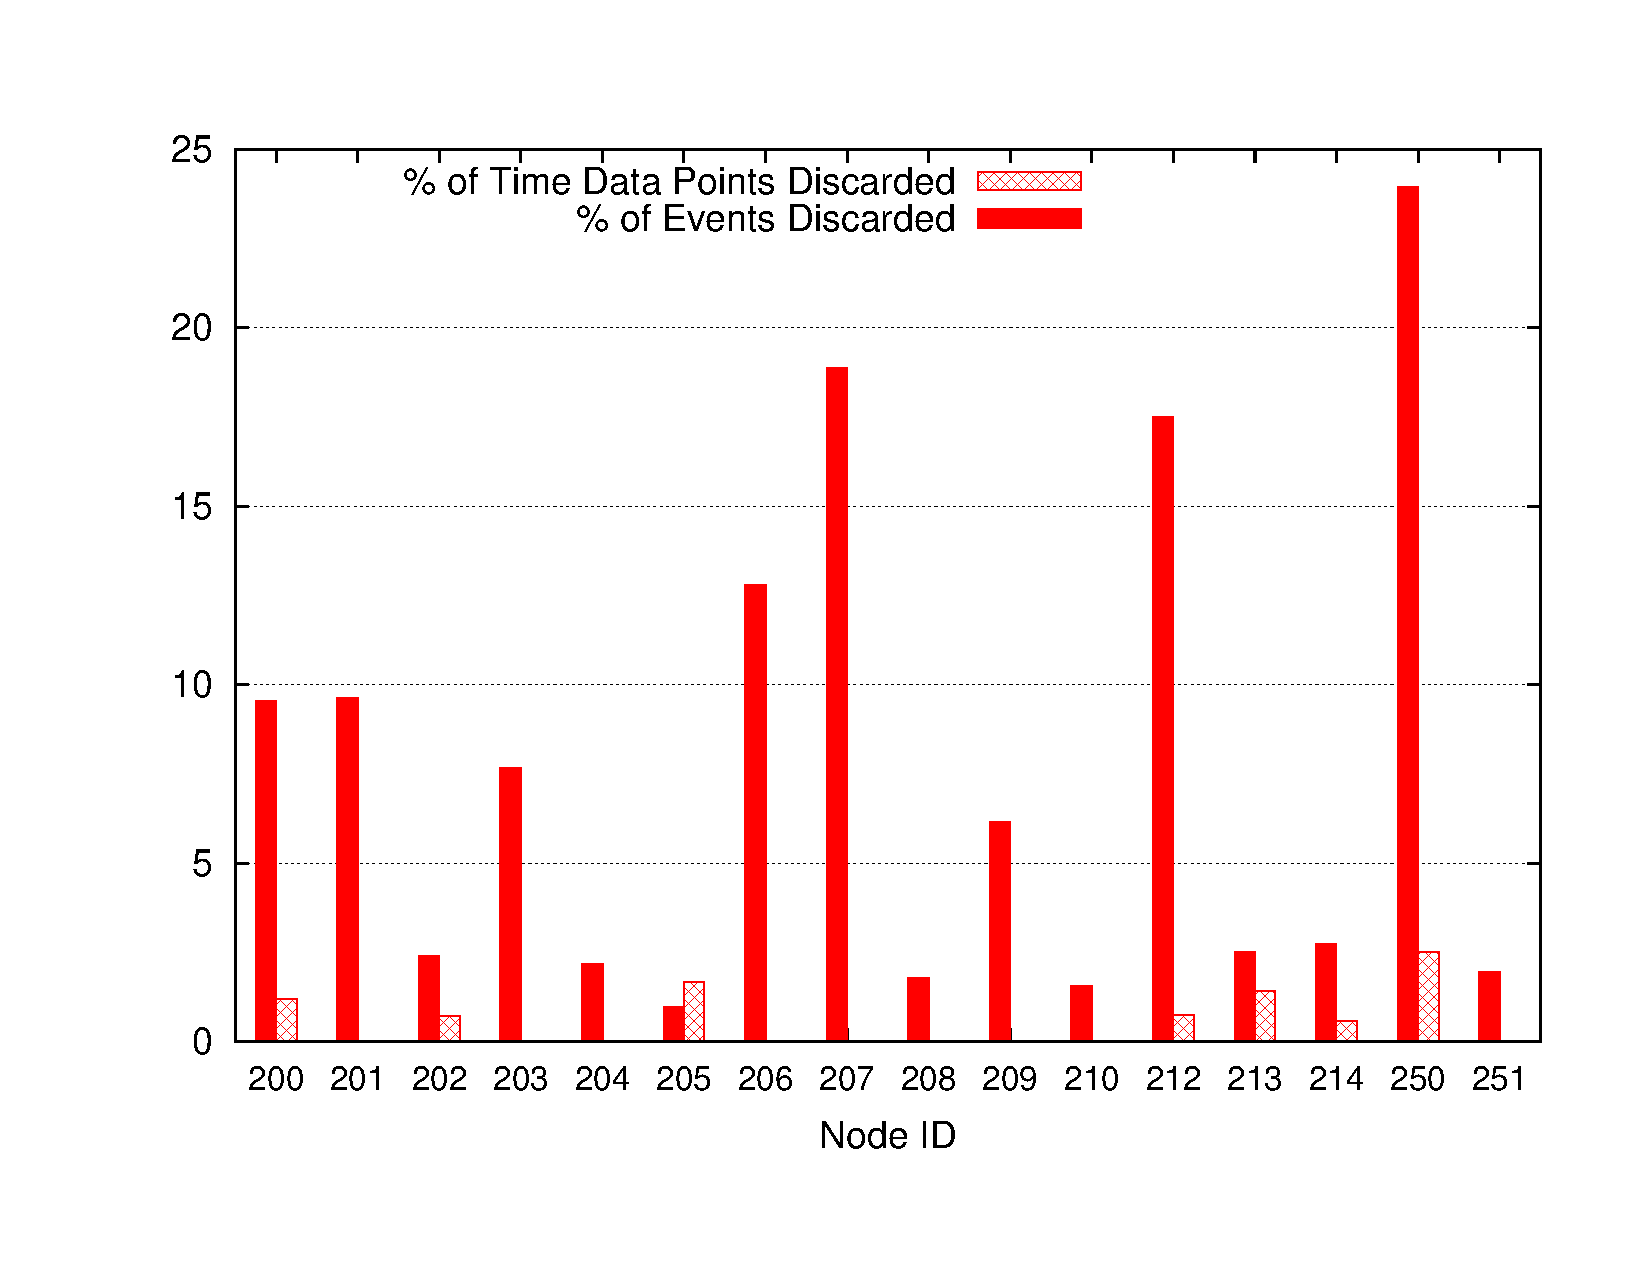
\includegraphics[width=\hsize]{./casestudy/figs/timing/ComparisonFigure/COMPARISONFIGURE.pdf}
%\end{center}
%\caption{\small{\bf Percentage of timestamps discarded by filtering versus
%percentage of events discarded because of timing failures:}
%{\em Overall, the filter rejected 7.9\% of the time 
%stamps reported by sensor nodes. Certain nodes, such as
%node~250, had an unusually large number of FTSP failures. However, the time
%rectification process can hide FTSP errors, as seen by the fact that overall
%we only had to discard 0.8\% of events because of bad timing.}}
%\label{fig-ftspdown}
%\end{figure}

\subsection{Timestamp rectification}
\label{section-timerectification}

\begin{figure}[t]
\begin{center}
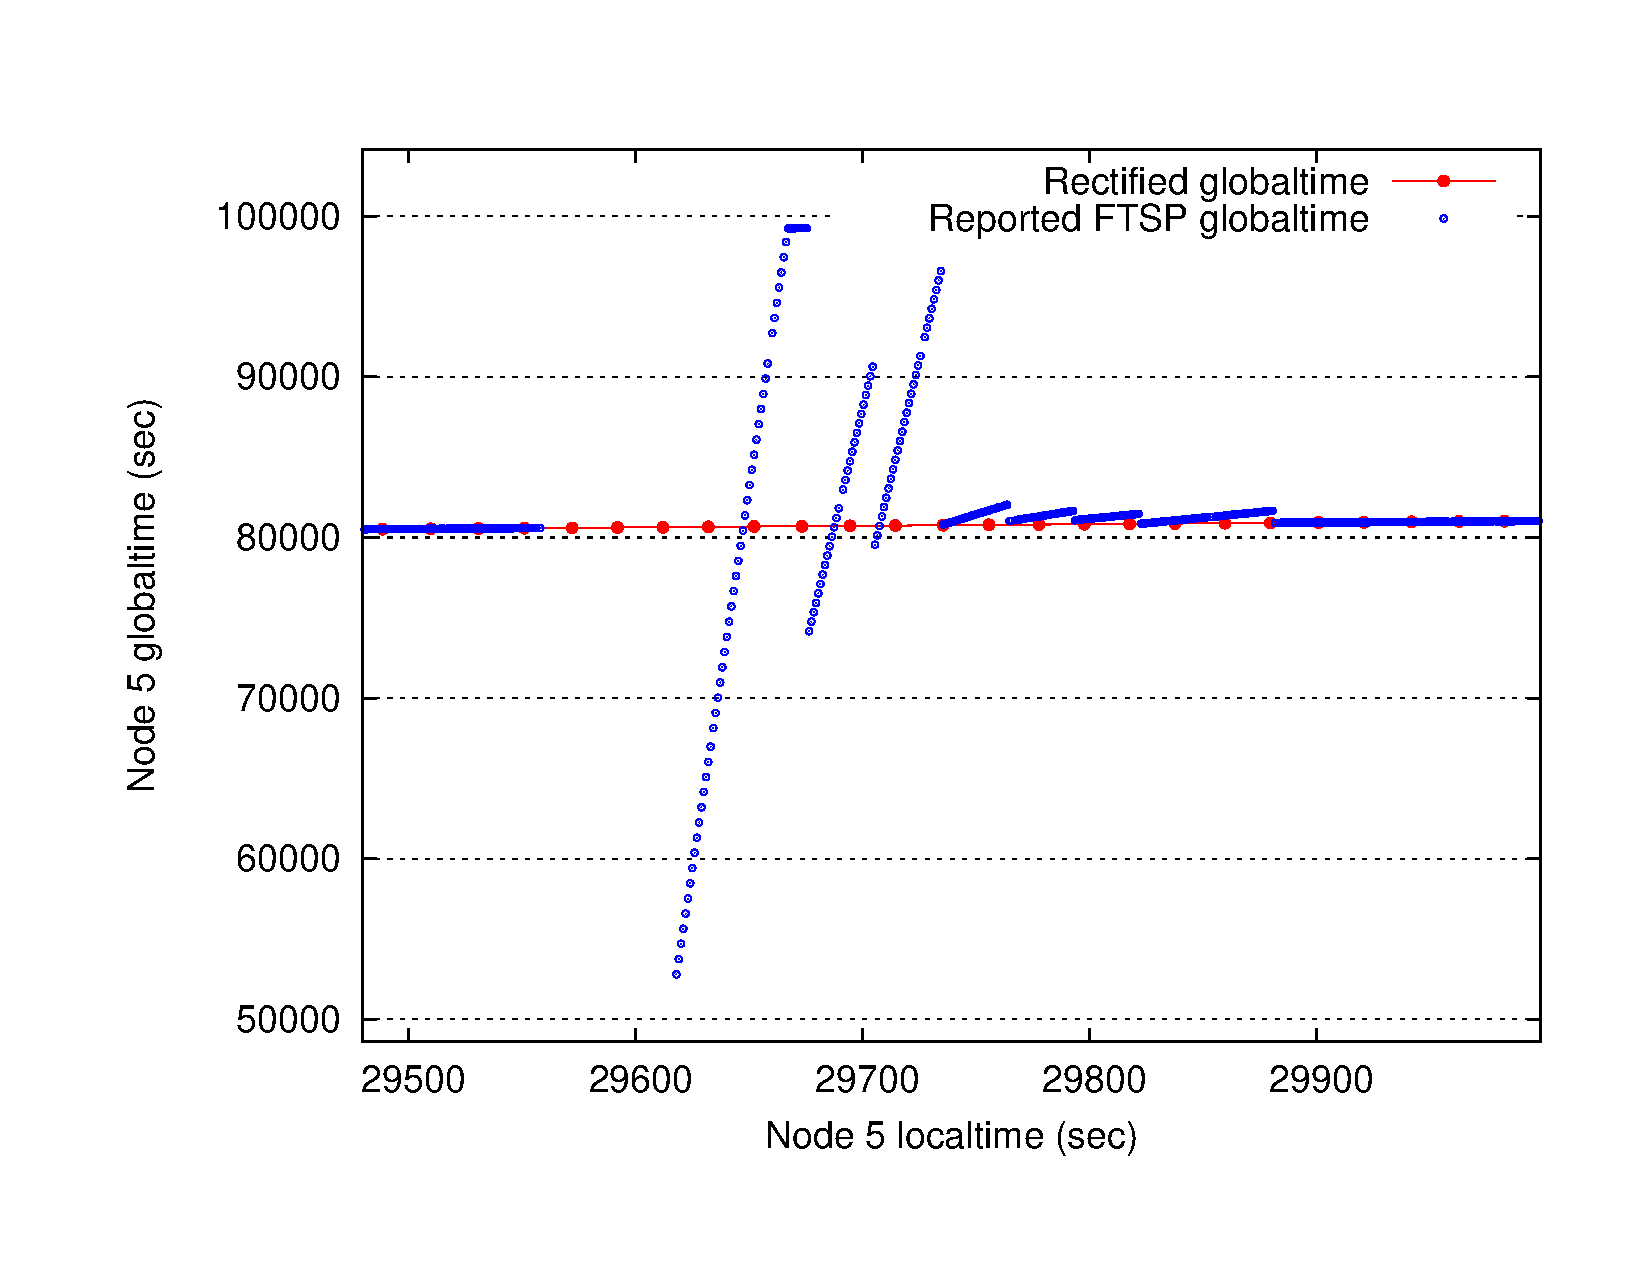
\includegraphics[width=\hsize]{./casestudy/figs/timing/MDW/rectification/rectify.pdf}
\end{center}
\caption{\small{\bf Time rectification example.}
{\em  The raw (LT, GT) pairs collected from the node show that
it experiences a period of FTSP instability.  The time rectification process
removes the errant timestamps creating an accurate mapping between LT
and GT created using a linear regression on the remaining
timestamps.}}
\label{fig-rectificationprocess}
\end{figure}

The goal of {\em time rectification} is to assign a GMT timestamp to each
sample in the recorded data. In order to do so, we build two models: one
mapping a node's local time to global time, and another mapping global time
to GMT. 
%
%\begin{figure}[t]
%\begin{center}
%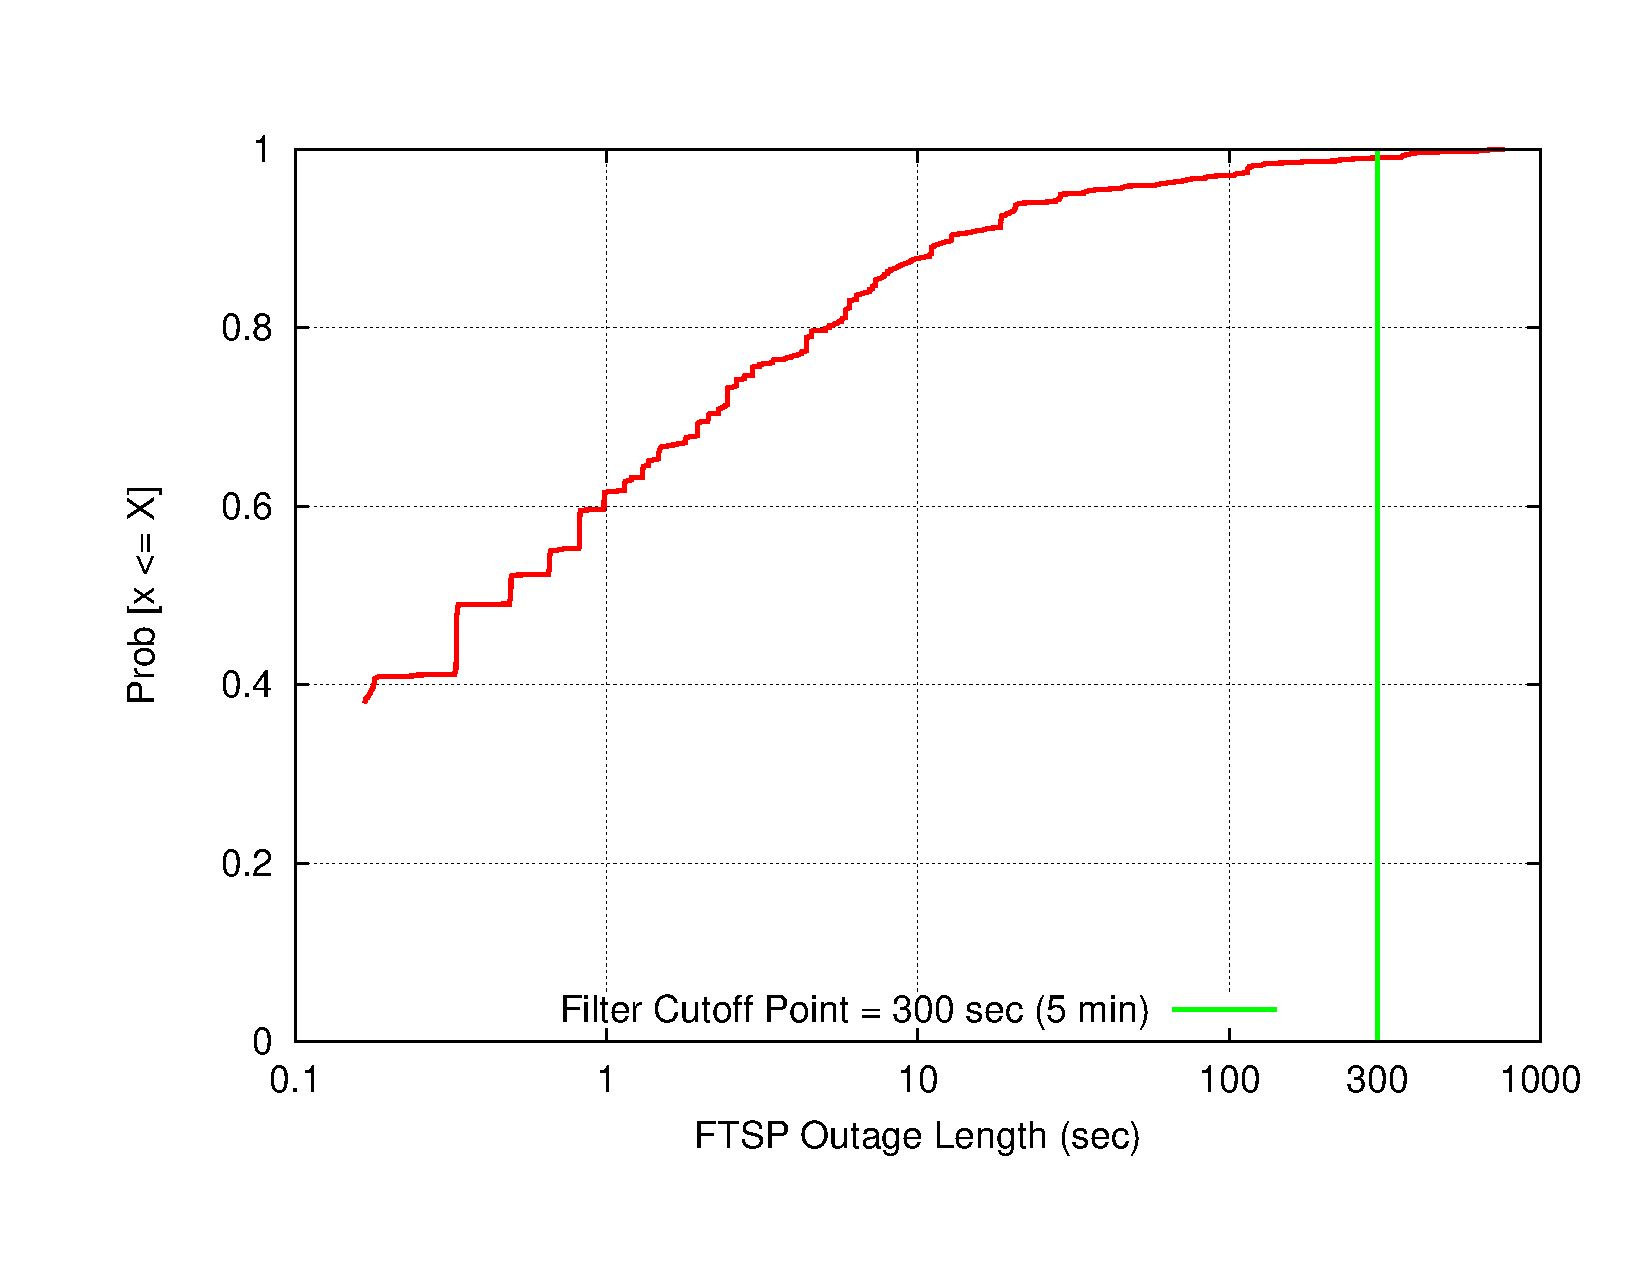
\includegraphics[width=\hsize]{./casestudy/figs/timing/FTSPRuns/FTSPDOWN-RUNS-CDF.pdf}
%\end{center}
%\caption{\small{\bf Run lengths for discarded timestamps:} {\em This is a CDF
%of the length of consecutive runs of timestamps discarded by our filter. As
%the figure shows, only 1\% of runs exceed our cutoff threshold of 5~minutes.
%The majority of runs are short and can be be bridged by the time
%rectification process.}}
%\label{fig-ftspdown-runs-cdf}
%\end{figure}
%
From those 
%the {\em (LT, GT)} information in the 
status messages that pass the
filter, we build a piecewise linear model mapping {\em LT} to {\em
GT} using a series of linear regressions. 
Models are constructed for each node separately, since local
times vary significantly between nodes.  Each regression spans up to
5~minutes of data and we initiate a new regression if the gap between
subsequent {\em (LT, GT)} pairs exceeds 5~minutes.  Each interval must
contain at least two valid status messages to construct the model.  We take
the {\em LT} value stored in each data block and use this model to recover
the corresponding {\em GT} value.

The next step is to map global time to GMT. Each of the GPS node's status
messages contain a {\em (GT, GMT)} pair. As above, we build a piecewise
linear model mapping {\em GT} to {\em GMT}, and apply this model to the {\em
GT} values for each data block. Finally, we assign a GMT value to each sample
contained in the block, using linear interpolation between the GMT values
assigned to the first sample in each block.  This process makes no
assumptions about sampling rate, which varies slightly from node to node due
to clock drift.

\subsection{Evaluation}
\label{timing-postdeployment}

Evaluating this time rectification process has proved
difficult, primarily because we have no ground truth for the timing
of the signals recorded in the field. However, by reproducing the deployment
conditions in the lab, we have been able to measure the accuracy of the
recovered timing in a controlled setting. In addition, as described earlier,
two GPS-synchronized data loggers were colocated with our sensor network,
providing us the opportunity to directly compare our time-rectified signals
with those recorded by conventional instrumentation.

Our first validation took place in the lab. Feeding the
output of a signal generator to both a miniature version of our sensor
network and to a Reftek~130 data logger allowed us to directly compare the data
between both systems.  The miniature network consisted of a single
sensor node, routing gateway, and GPS receiver node. The same software was
used as in the field deployment. The Reftek~130 logs data
to a flash memory card and timestamps each sample using its own GPS receiver.
%The Reftek~130 is commonly used in volcano field studies and its timing
%accuracy has been extensively validated.

The results showed a consistent 15~ms offset between the time-rectified 
signals recorded by the sensor node and the Reftek data logger.  
We discovered that this offset was due to delays introduced by 
the digital filtering performed by the
ADC on our sensor board (see Section~\ref{sec-hardware}). Adjusting for this
delay resulted in an indiscernible offset between the sensor node and 
Reftek signals. While this experiment does not reproduce the full 
complexity of our deployed network, it does serve as a baseline for 
validation.

In the second lab experiment, we set up a network of 7~sensor nodes in a
6-hop linear topology. The topology is enforced by software, but all nodes
are within radio range of each other, making it possible to stimulate all
nodes simultaneously with a radio message.  Each node samples data and sends
status messages using the same software as the field deployment. The FTSP
root node periodically transmits a beacon message. On reception of the
beacon, each node records the FTSP global timestamp of the message reception
time (note that reception of the beacon message is not limited by the
software-induced topology).  Because we expect all nodes to receive this
message at the same instant, modulo interrupt latency jitter, we expect the
FTSP time recorded by each node to be nearly identical. The FTSP root also
records the time that the beacon was transmitted, accounting for MAC delay.
The experiment ran for 34~hours, during which time FTSP experienced
instabilities similar to those seen during our deployment.

\begin{figure}
\begin{tabular}{|lll|} \hline
                  & {\bf Raw error} & {\bf Rectified error} \\ \hline
{\bf  1 hop}, 50th percentile & 1.52 ms & 1.42 ms \\ 
{\bf 1 hop}, 90th percentile & 9.86 ms & 6.77 ms \\ \hline 
{\bf 6 hops}, 50th percentile & 2.63 ms & 2.18 ms \\ 
{\bf 6 hops}, 90th percentile & 13.5 ms & 6.8 ms \\ \hline 
\end{tabular} \\
\vspace{2ex}
\caption{\small {\bf Timestamp errors in a 6-hop lab testbed:}
{\em This table shows the 50th and 90th-percentile timing errors
on both the raw FTSP timestamps, and rectified timestamps.}}
\label{fig-time-rect-lab}
\end{figure}

This allows us to compare the {\em true} global time of each beacon message
transmission and the {\em apparent} global time on each receiving node, both
before and after subjecting the data to our time rectification process.  We
call the difference between the true and apparent times the {\em timestamp
error}. Figure~\ref{fig-time-rect-lab} shows the results for nodes one and
six hops away from the FTSP root.  After rectification, 99.9\% of the errors
for the one-hop node and 93.1\% of the errors for the six-hop node fall
within our 10~ms error envelope.

%\begin{figure}[t]
%\begin{center}
%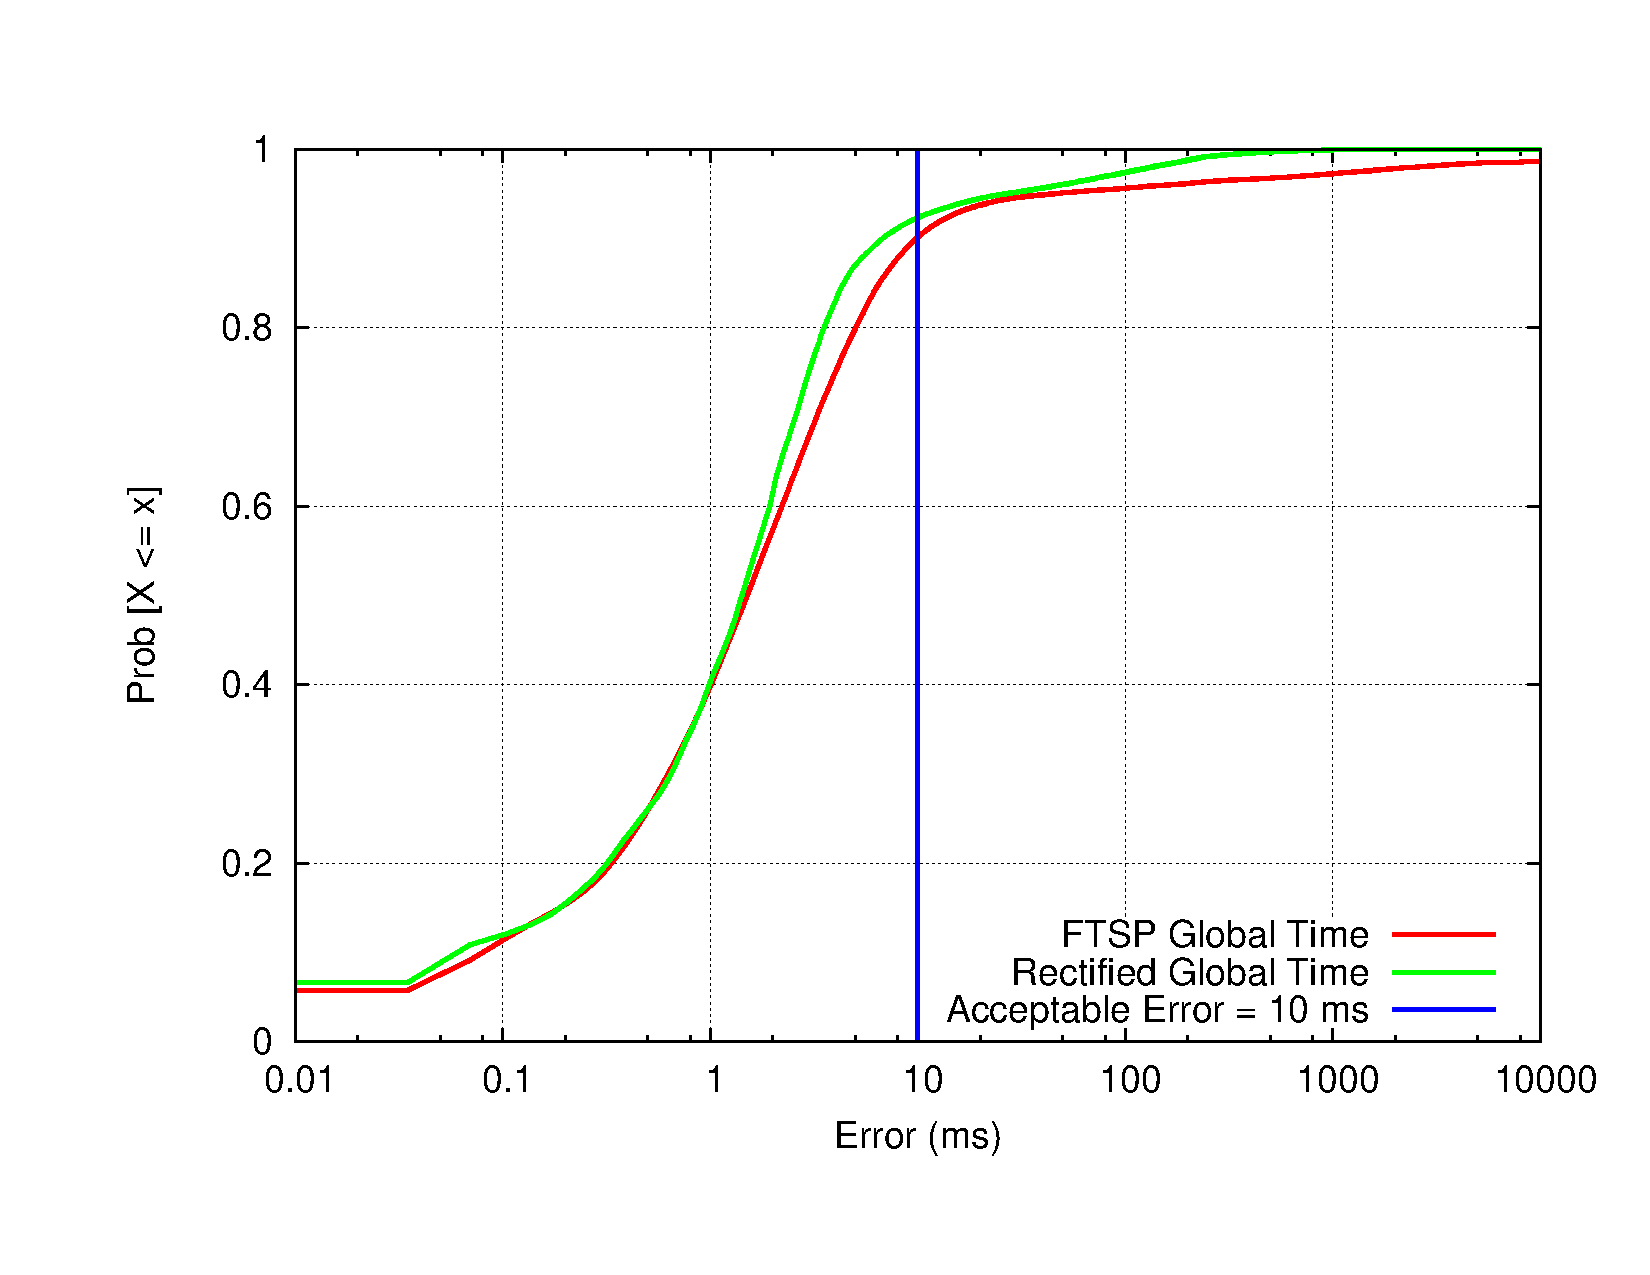
\includegraphics[width=\hsize]{./casestudy/figs/timing/TelosLabNew/FTSPVMAPPEDNODE0.pdf}
%{\small {\bf (a, 1 hop)}}
%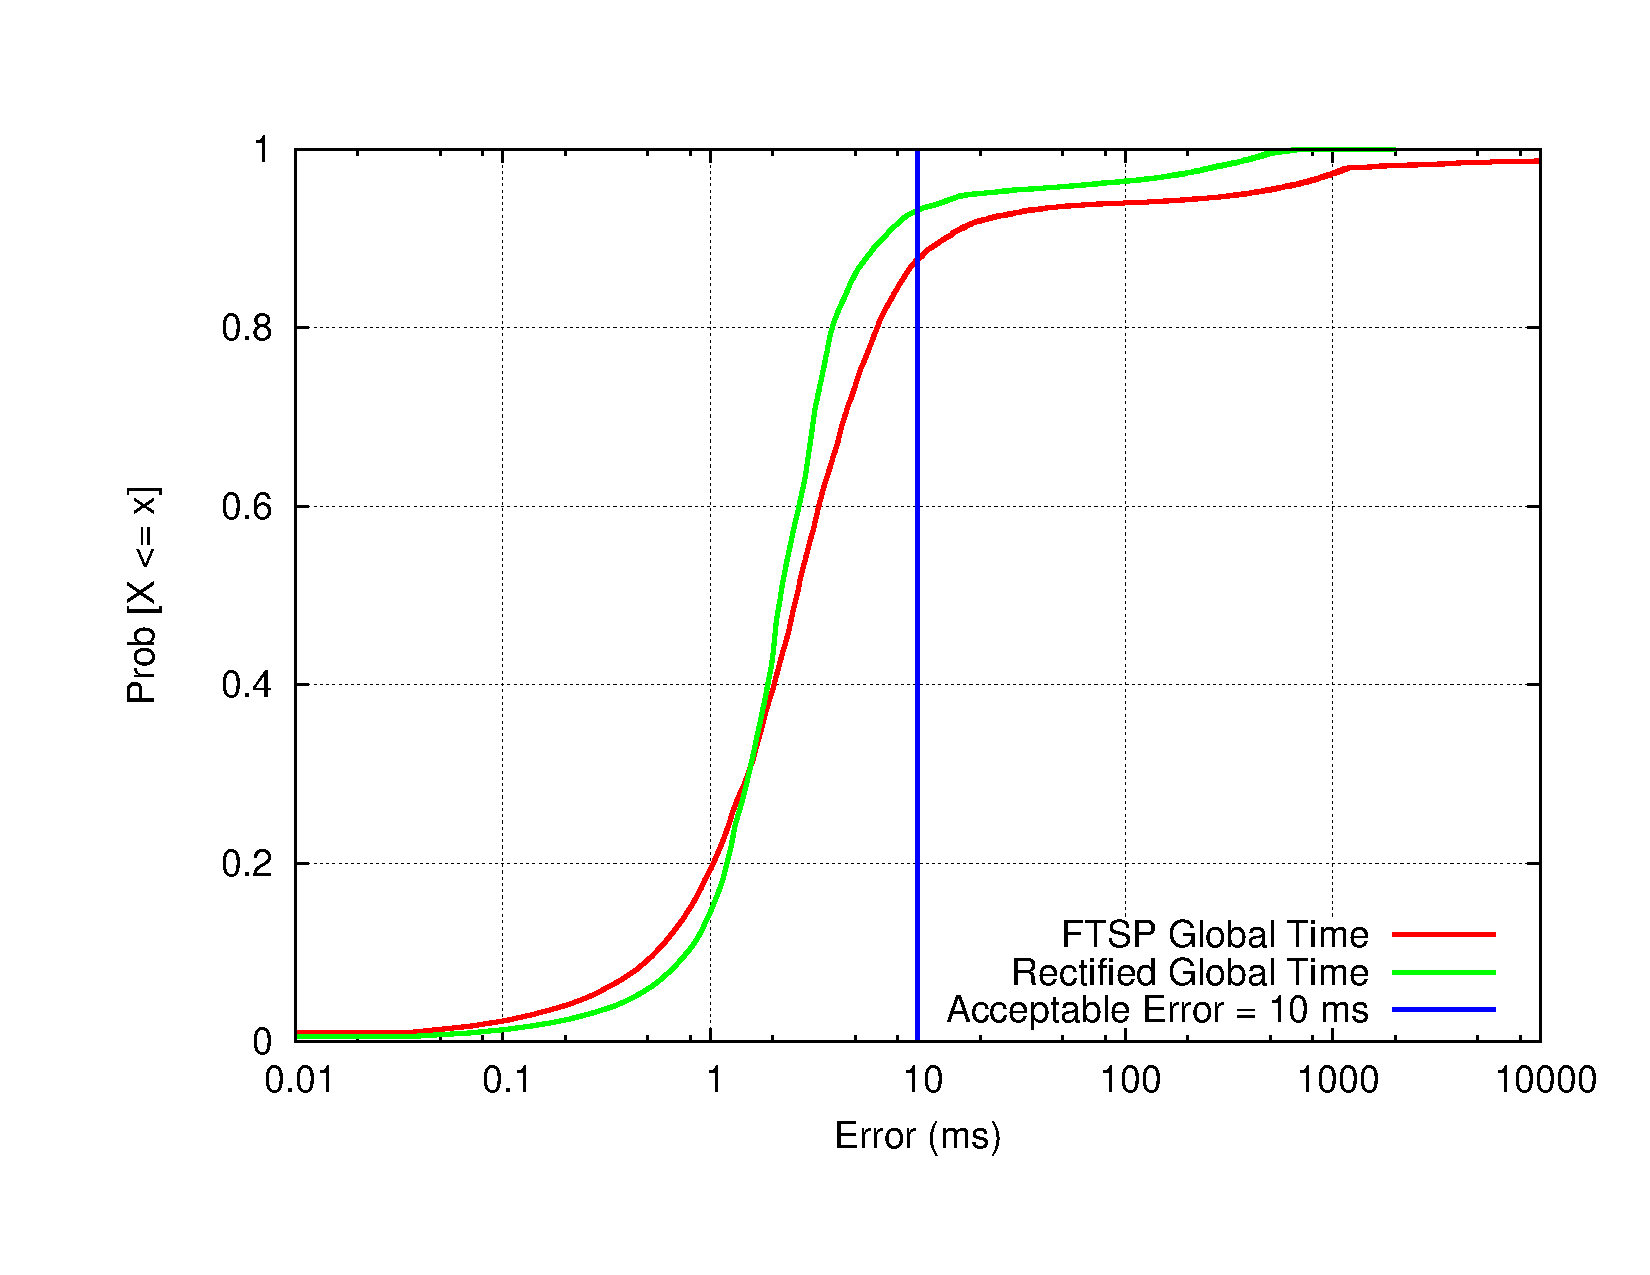
\includegraphics[width=\hsize]{./casestudy/figs/timing/TelosLabNew/FTSPVMAPPEDNODE6.pdf}
%{\small {\bf (b, 6 hops)}}
%\end{center}
%\caption{\small{\bf Testbed Comparison of FTSP and Time Rectification Errors}
%{\em During the experiment described in Section~\ref{timing-postdeployment}
%we used periodic heartbeat messages to collect synchronous local time, global
%time pairs across the network.  These graphs show the distribution of the
%FTSP error and the mapping error with respect to the ``true'' global time,
%that is the stamp recorded on the broadcast node when it sent the message,
%for two nodes.  Figure (a) shows the distribution for the node 1 hop away
%  from the root of the FTSP tree.  For this node, 96.4\% of the FTSP global
%  timestamps and 99.9\% of the mapped global timestamps were within 10~ms of
%  the true global time. Figure (b) shows the same distribution for the node 6
%  hops from the root.  For this node, 87.6\% of the FTSP global timestamps
%  and 93.1\% of the mapped global timestamps were within 10~ms of the true
%  global time. We had a difficult time reproducing the long periods of FTSP
%  instability experienced in the field in the testbed setting.}}
%\label{fig-benchtest}
%\end{figure}

% 20 Apr 2006 : GWA : UNUSED FIGURES.

%\begin{figure}[t]
%  \begin{small}
%    \begin{center}
%      \begin{tabular}{|cc|} \hline
%        {\bf Event} & {\bf Shift} \\ \hline
%2005-08-13\_03.38.08 & 29 \\
%2005-08-13\_06.16.46 & -45 \\
%2005-08-13\_08.17.51 & 29 \\
%2005-08-13\_15.24.58 & -36 \\
%2005-08-15\_04.48.27 & -43 \\
%2005-08-15\_07.07.52 & 46 \\
%2005-08-15\_09.11.28 & -29 \\
%2005-08-15\_16.04.37 & 48 \\
%2005-08-16\_04.04.56 & -21 \\
%2005-08-16\_09.45.14 & 15 \\
%2005-08-17\_05.07.31 & -26 \\
%2005-08-17\_14.00.43 & -26 \\
%2005-08-17\_16.48.26 & -71 \\
%2005-08-18\_00.52.31 & 11 \\
%2005-08-18\_03.43.05 & 41 \\
%2005-08-18\_04.54.30 & 23 \\
%2005-08-18\_06.26.50 & 19 \\
%2005-08-18\_17.59.49 & 45 \\
%2005-08-18\_21.33.01 & 8 \\
%2005-08-19\_00.16.22 & -7 \\
%2005-08-19\_01.52.09 & -25 \\
%2005-08-19\_02.33.30 & -58 \\
%2005-08-15\_19.29.08 & 48 \\
%2005-08-17\_00.22.39 & -55 \\
%2005-08-17\_02.09.47 & -27 \\
%2005-08-18\_13.28.54 & 9 \\
%2005-08-18\_14.23.06 & 25 \\
%2005-08-18\_15.31.06 & -42 \\
%        \hline
%      \end{tabular}
%    \end{center}
%  \end{small}
%\caption{\small{\bf Hand-picked Shifts Between Node 213 and Reftek} {\em For
%each event that we had signals from both Node 213 and the RVEN, the Reftek
%station located nearby, we used {\tt MATLAB}'s {\tt xcorr} function to
%produce some possible time shifts between each signal.  We then examined each
%shift by hand to pick the best one.  An example of this process can be seen
%in Figure~\ref{fig-rvenv213}. This table shows the shifts for all events for
%which we had paired data. As can be seen most are under 50~ms, the greatest
%possible shift possible given the distance between the stations.}}
%\label{fig-rvenv213table}
%\end{figure}

%\begin{figure}[t]
%\begin{center}
%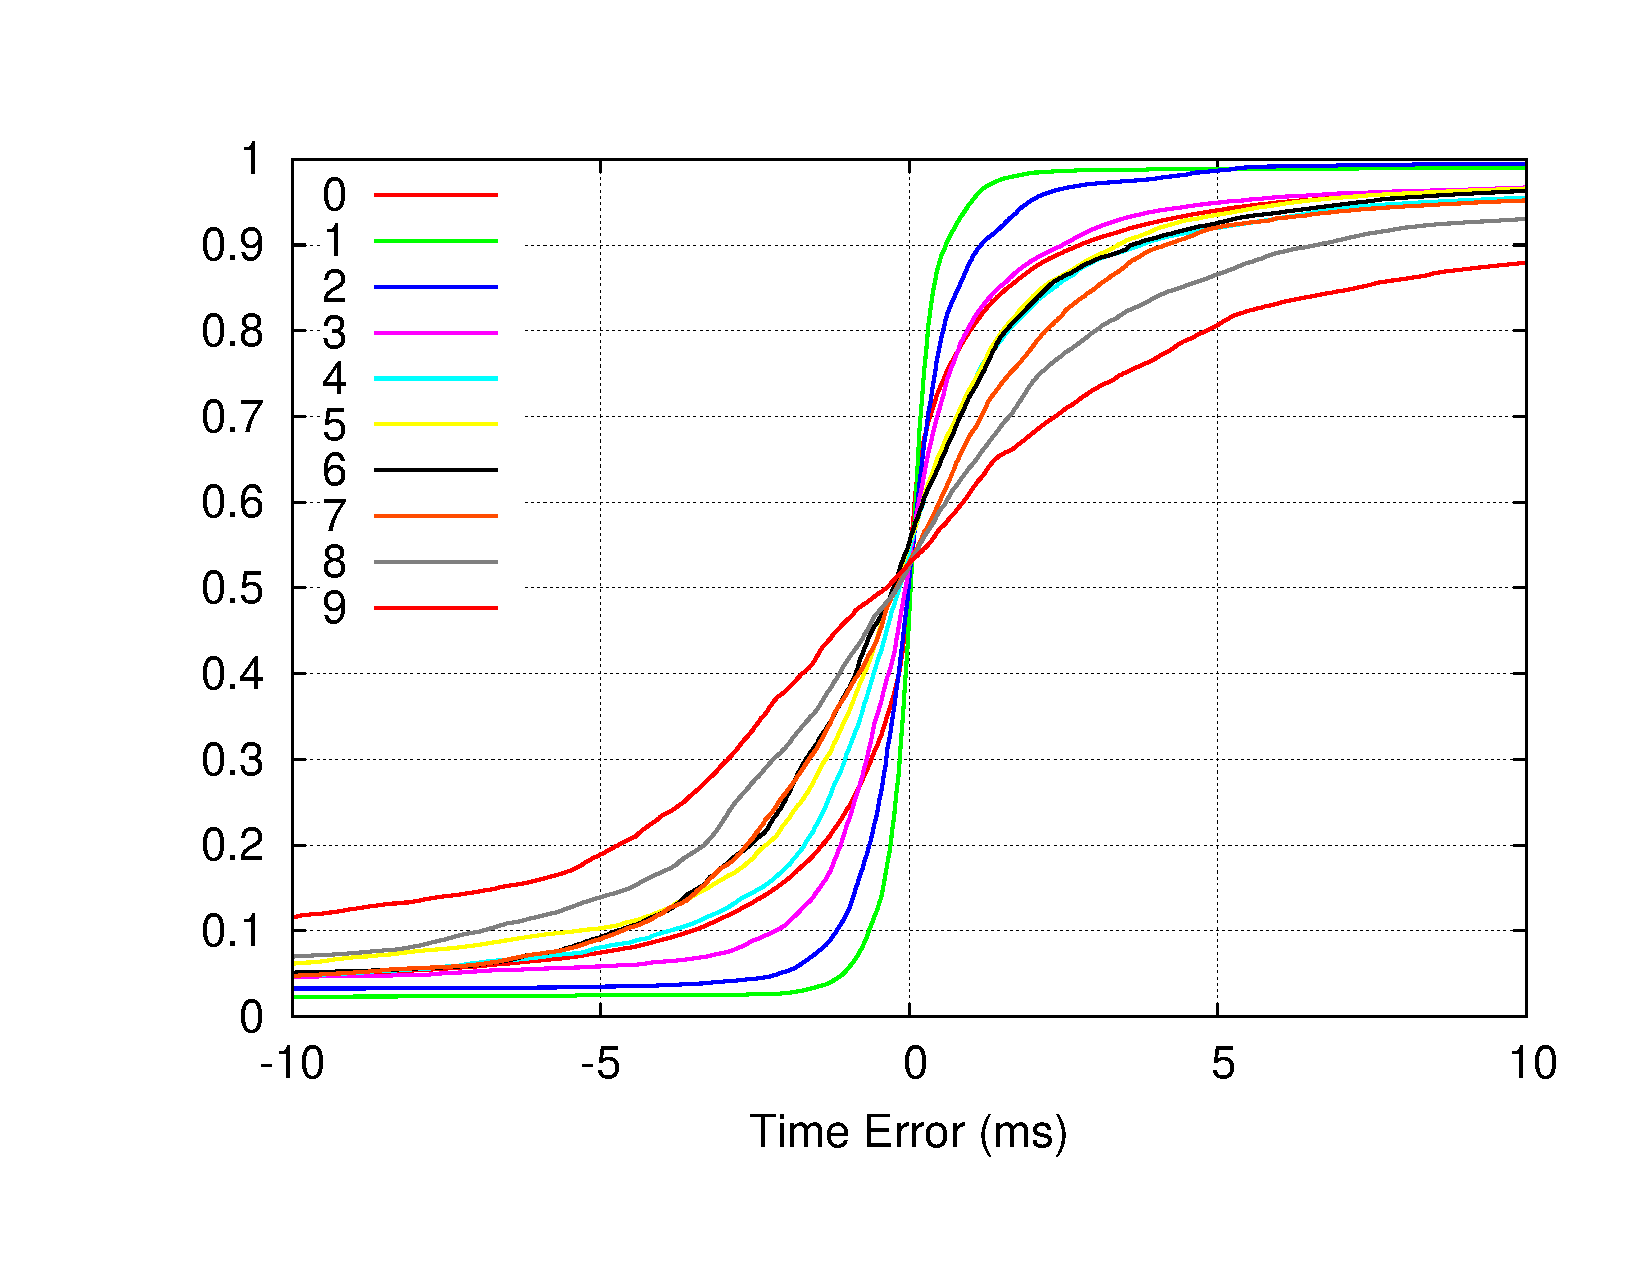
\includegraphics[width=\hsize]{./casestudy/figs/timing/TelosLabTiming/MAPPINGERROR.pdf}
%\end{center}
%\caption{\small{\bf Distribution of Bench Test FTSP Mapped Global to Reported
%Global Time Errors}
%{\em \GWAnote{I don't think that this graph should be in the paper, so I'm
%not commenting it.  The rest of this stuff is confusing enough and this
%doesn't say much because the errors are not additive!}}}
%\label{fig-mappingerror}
%\end{figure}

%\begin{figure}[t]
%\begin{center}
%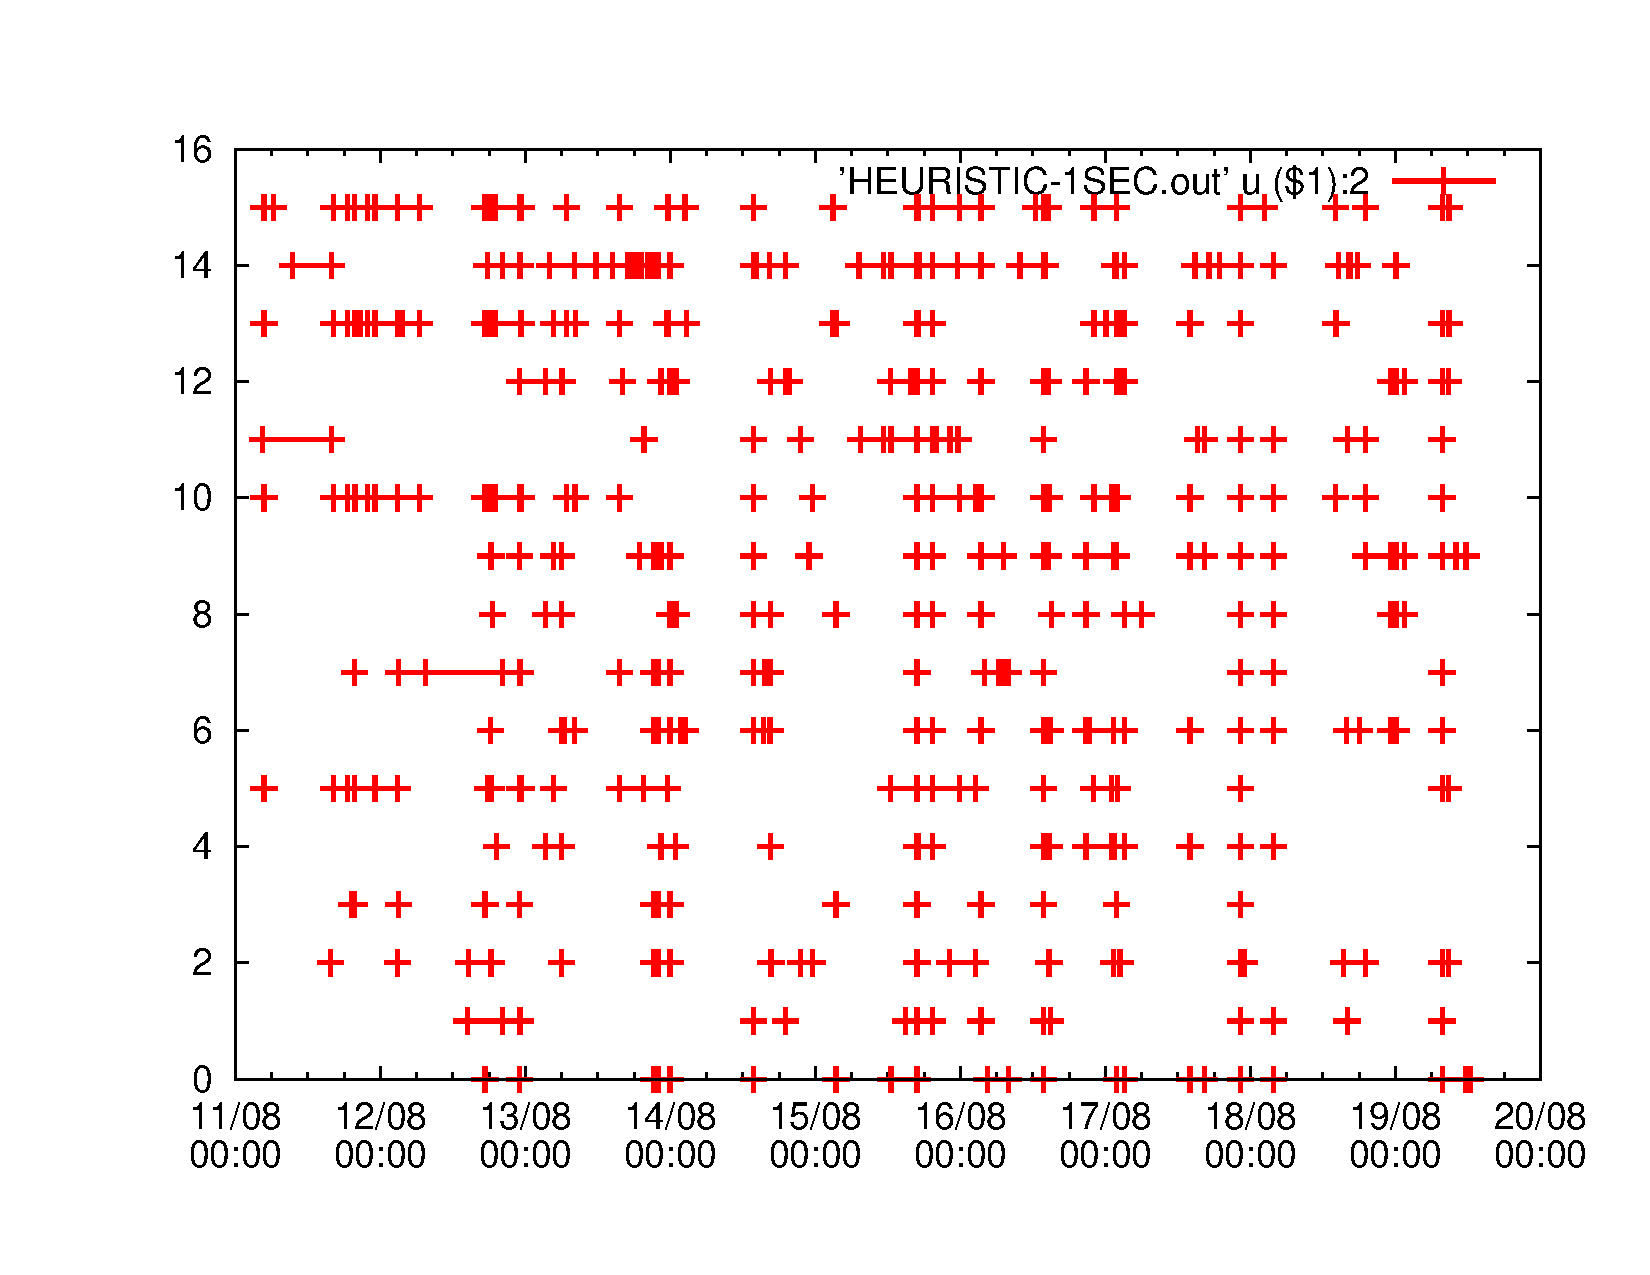
\includegraphics[width=\hsize]{./casestudy/figs/timing/TimingHeuristicRuns/HEURISTIC-1SEC.pdf}
%\end{center}
%\caption{\small{\bf Time Location of Consecutive Runs of Timestamps with
%Heuristic Time Difference of Over 1 second}
%{\em \GWAnote{This probably won't be in the paper either.}}}
%\label{fig-heuristic-1sec}
%\end{figure}

%\begin{figure}[t]
%\begin{center}
%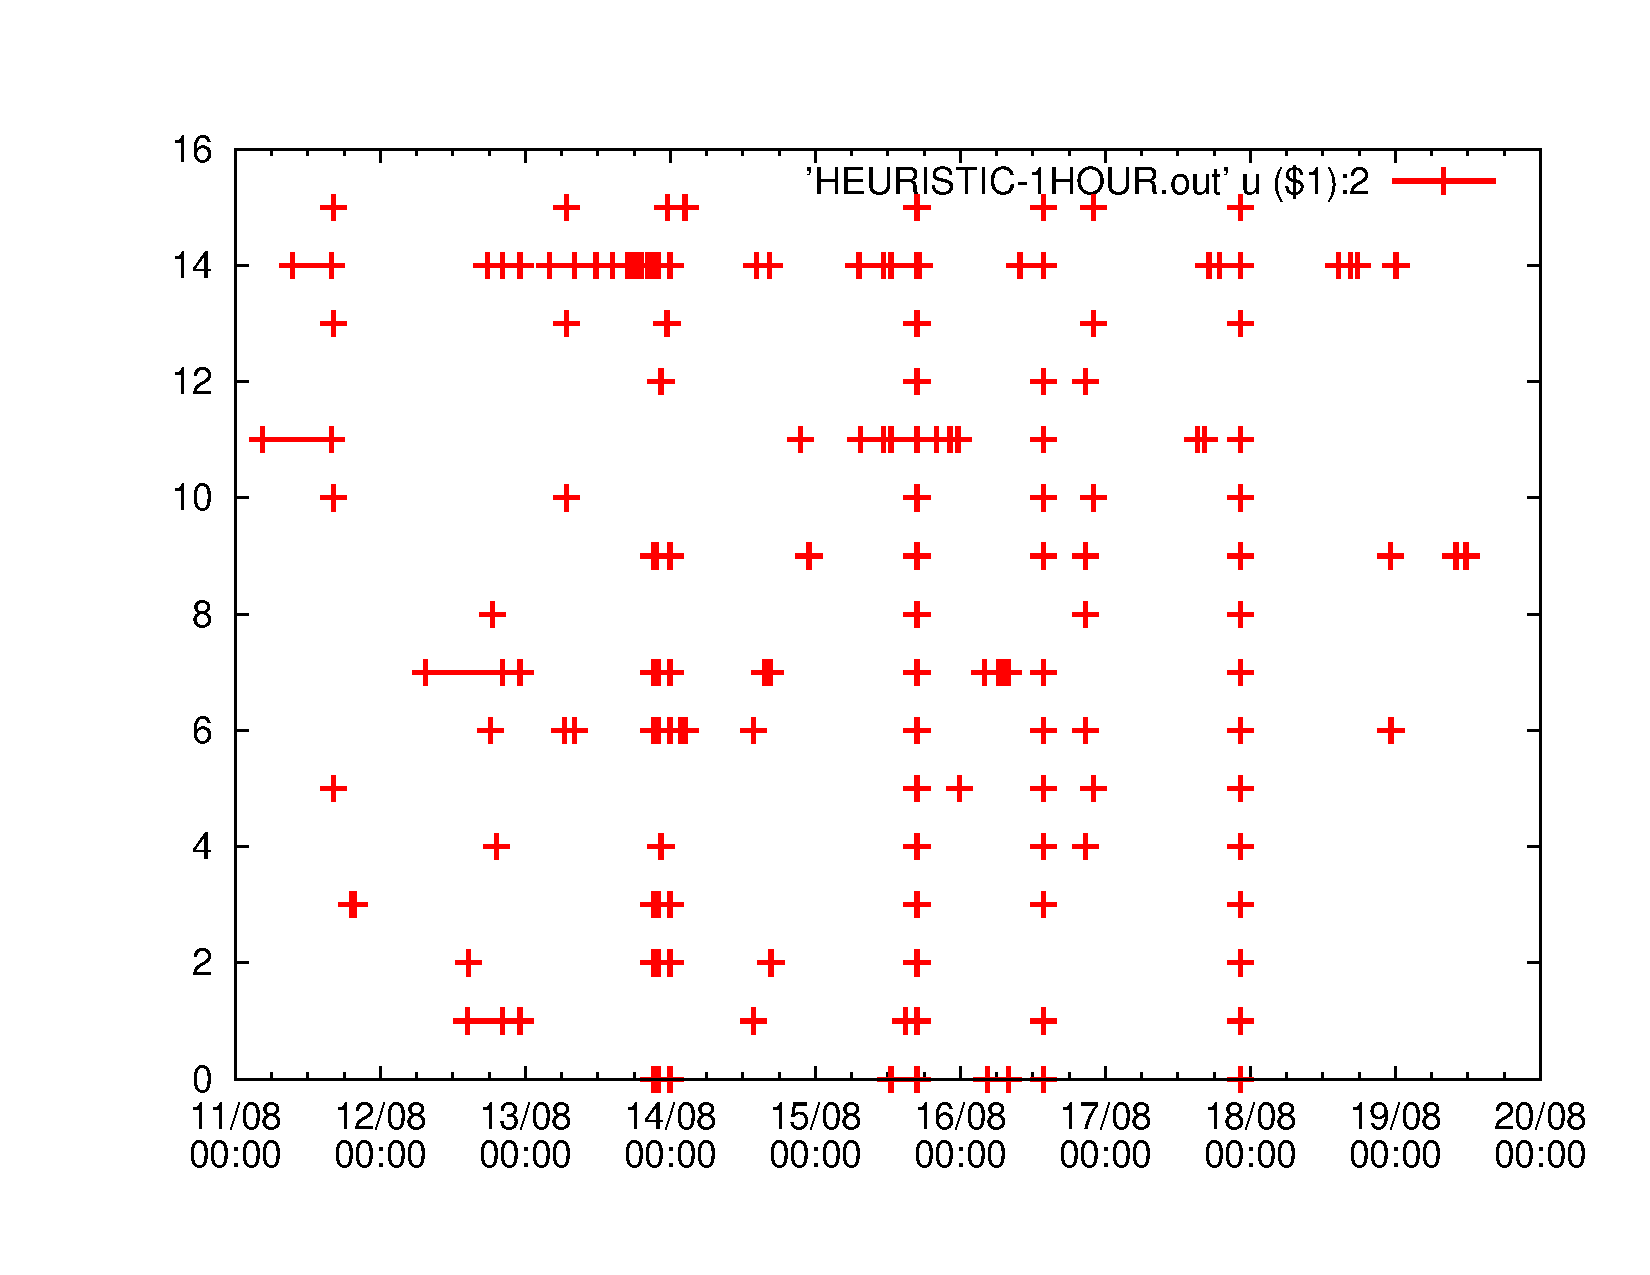
\includegraphics[width=\hsize]{./casestudy/figs/timing/TimingHeuristicRuns/HEURISTIC-1HOUR.pdf}
%\end{center}
%\caption{\small{\bf Time Location of Consecutive Runs of Timestamps with
%Heuristic Time Difference of Over 1 hour}
%{\em Marked regions on this time-series indicate periods during with a given
%nodes time data points had a heuristic error of over 1 hour.  There are
%several small, well-correlated periods at periodic intervals caused by clock
%rollover on the root node.  Larger intervals show periods when FTSP errors
%prevented nodes from accurated time stamping data.  As shown in Figure FIXME
%and Figure FIXME this occured more often for certain nodes than for others.
%\GWAnote{I think that if we keep one of these it should be this one.  1 hour
%is obviously a bad heuristic diff and this graph looks a lot like the 60
%second one.}}}
%\label{fig-heuristic-1hour}
%\end{figure}

%\begin{figure}[t]
%\begin{center}
%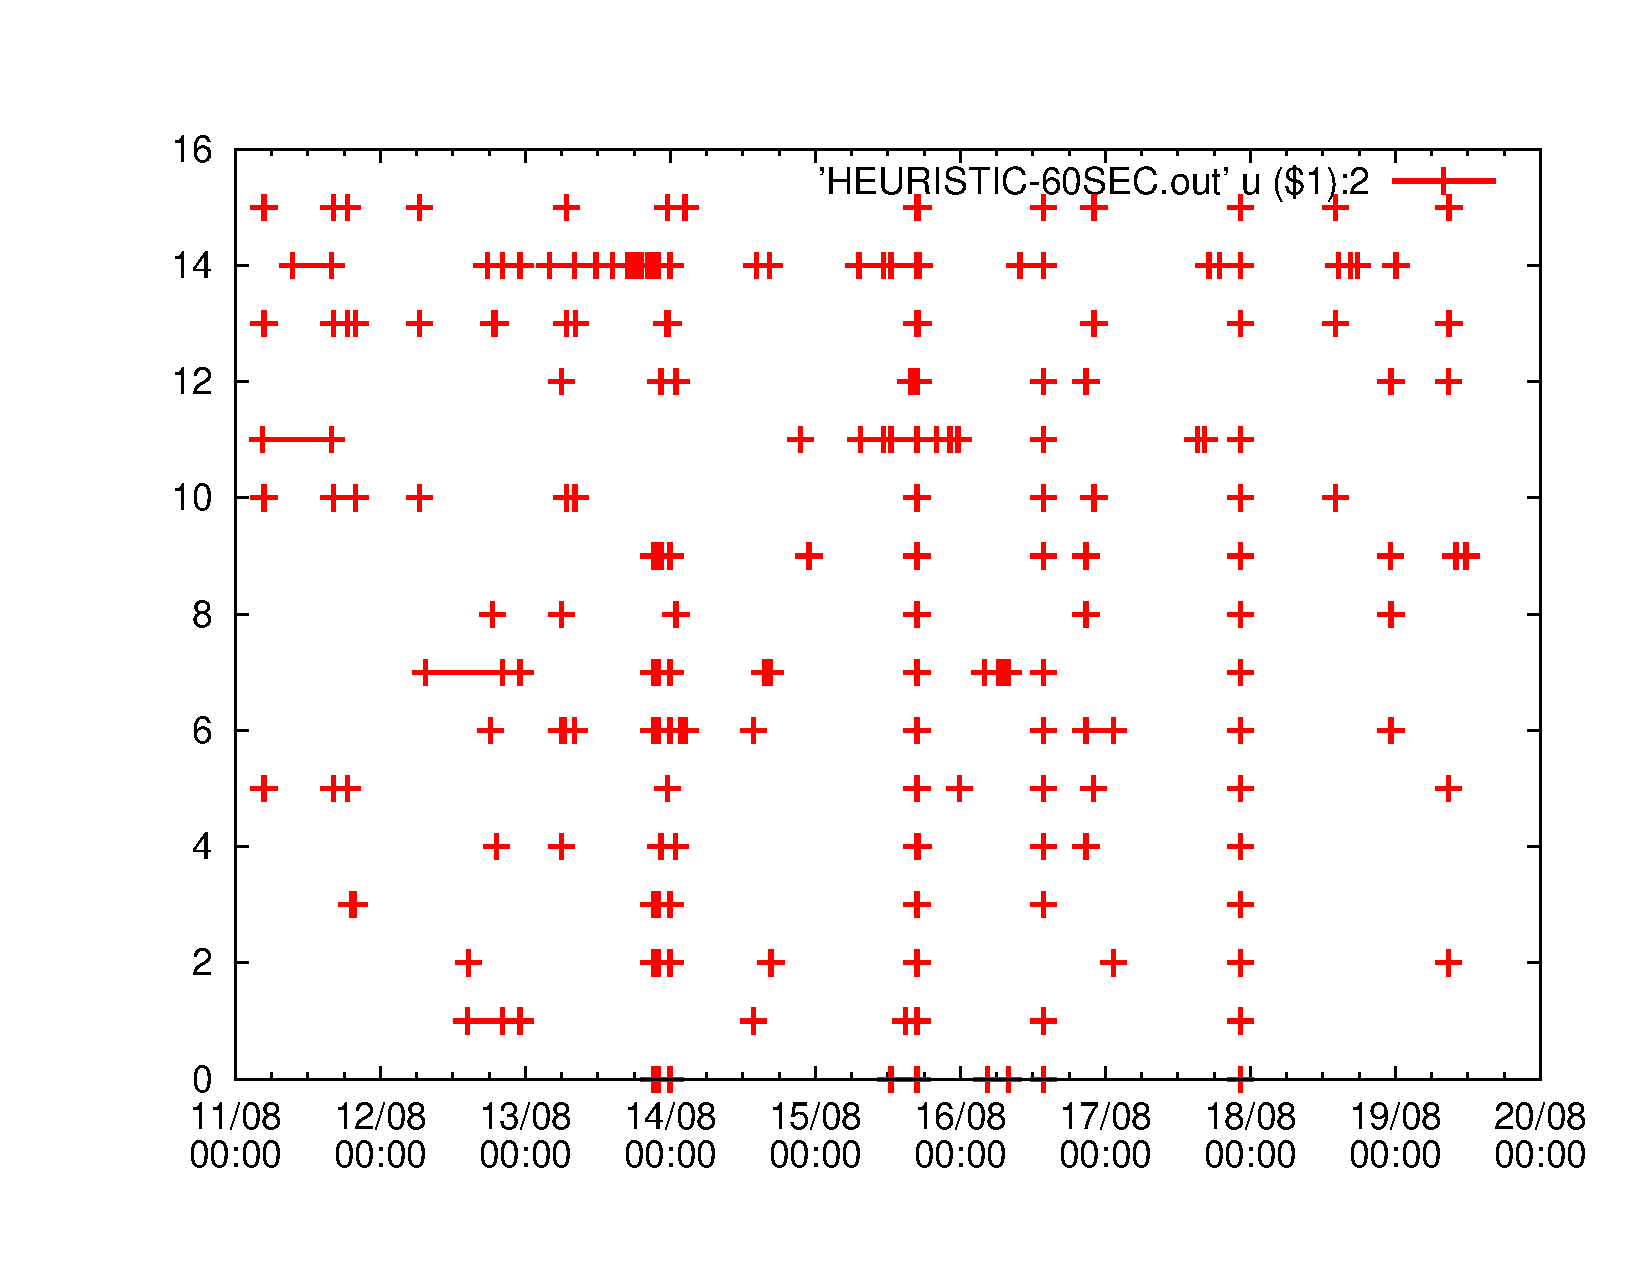
\includegraphics[width=\hsize]{./casestudy/figs/timing/TimingHeuristicRuns/HEURISTIC-60SEC.pdf}
%\end{center}
%\caption{\small{\bf Time Location of Consecutive Runs of Timestamps with
%Heuristic Time Difference of Over 60 seconds}
%{\em \GWAnote{Don't think that we need this one either.}}}
%\label{fig-heuristic-60sec}
%\end{figure}

%\begin{figure}[t]
%\begin{center}
%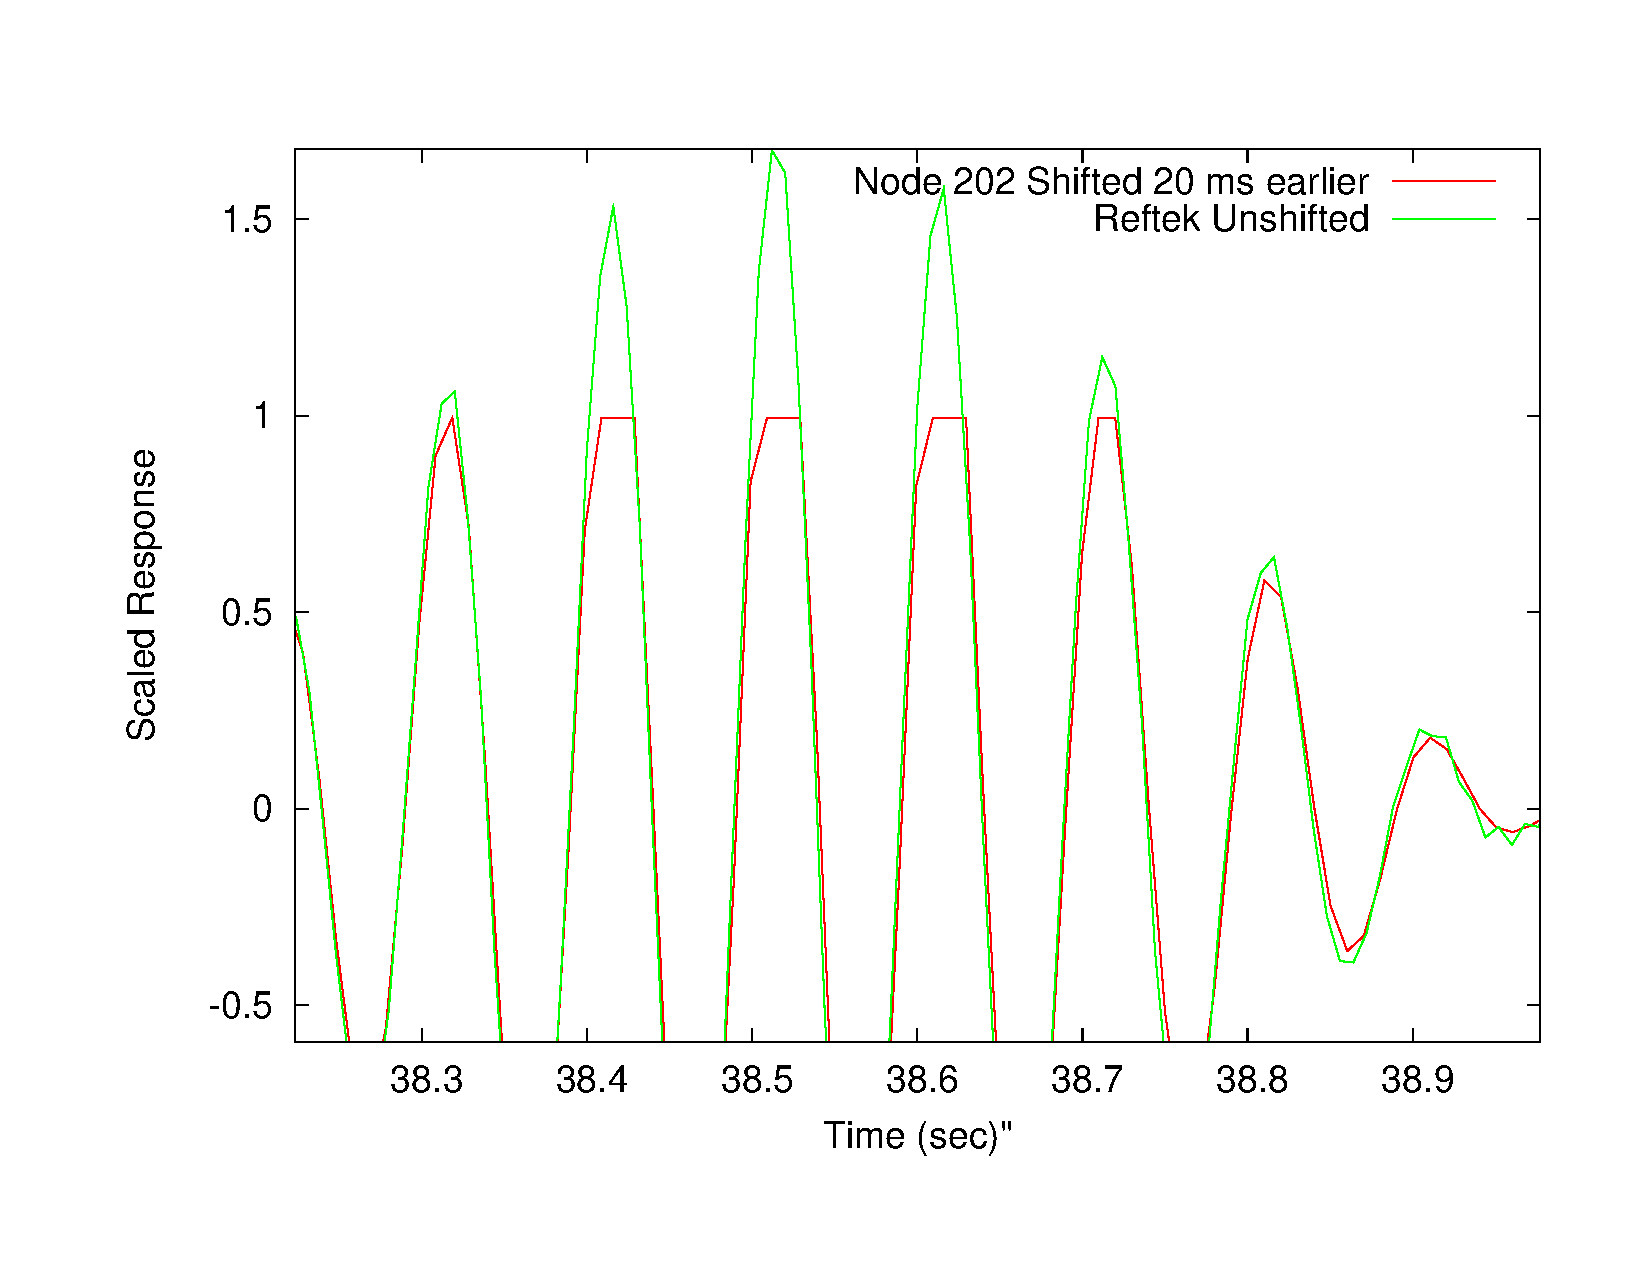
\includegraphics[width=\hsize]{./casestudy/figs/timing/FirstReftekComparison/COMPARISON-SHIFTED.pdf}
%\end{center}
%\caption{\small{\bf Reftek Side-by-side Test Signals with 15 ms Shift Applied}
%{\em This graph shows the output of the Reftek side-by-side test (described
%in more detail in Section FIXME) after applying a 15ms time shift as
%suggested by the engineers at Analog Devices.}}
%\label{fig-comparisonshifted}
%\end{figure}

%\begin{figure}[t]
%\begin{center}
%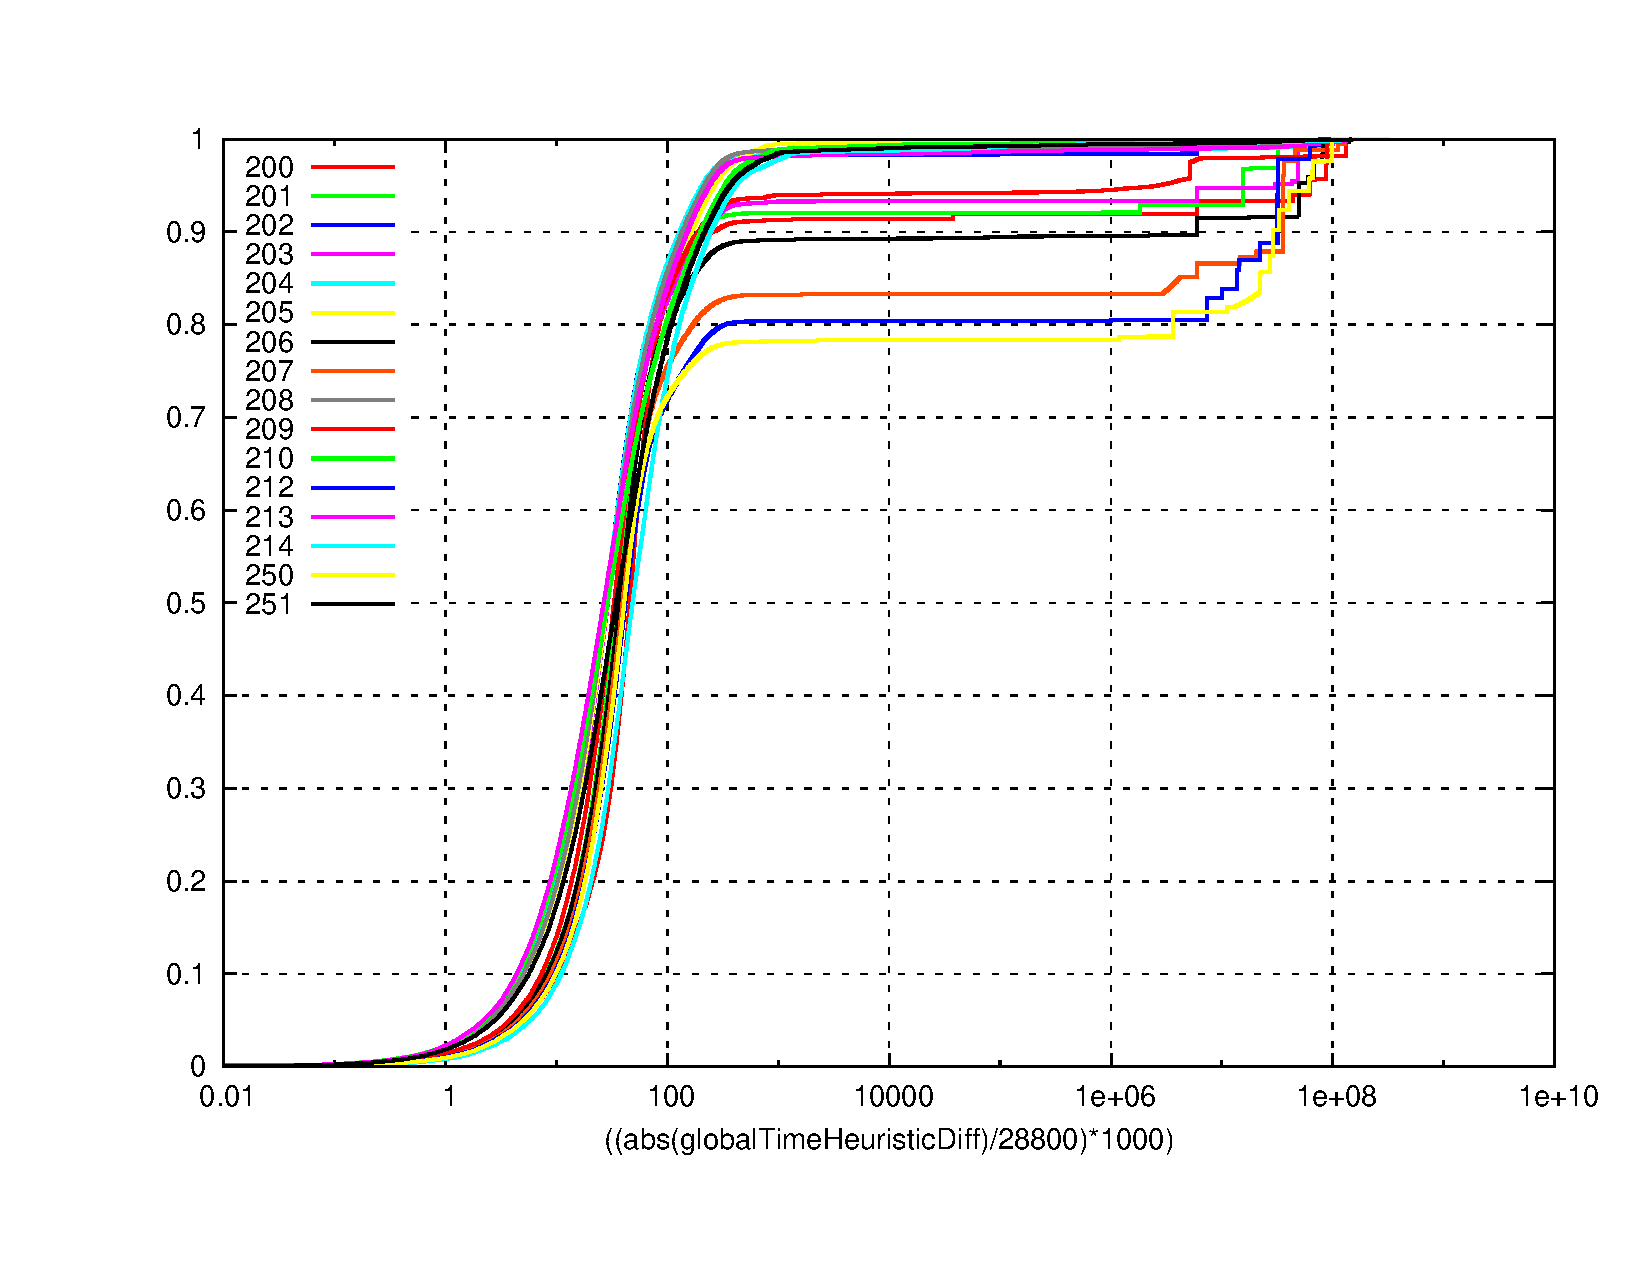
\includegraphics[width=\hsize]{./casestudy/figs/timing/TimingHeuristicDiffs/TIMINGHEURISTICABS.pdf}
%\end{center}
%\caption{\small{\bf Distribution of Absolute Heuristic Time Difference by
%Node ID} {\em The graph shows the distribution of absolute heuristic time
%differences (as described in Section~\ref{}).  The time rectification process discards
%points with a difference of over 1000ms (1 sec).}}
%\label{fig-timingheuristicabs}
%\end{figure}

%\begin{figure}[t]
%\begin{center}
%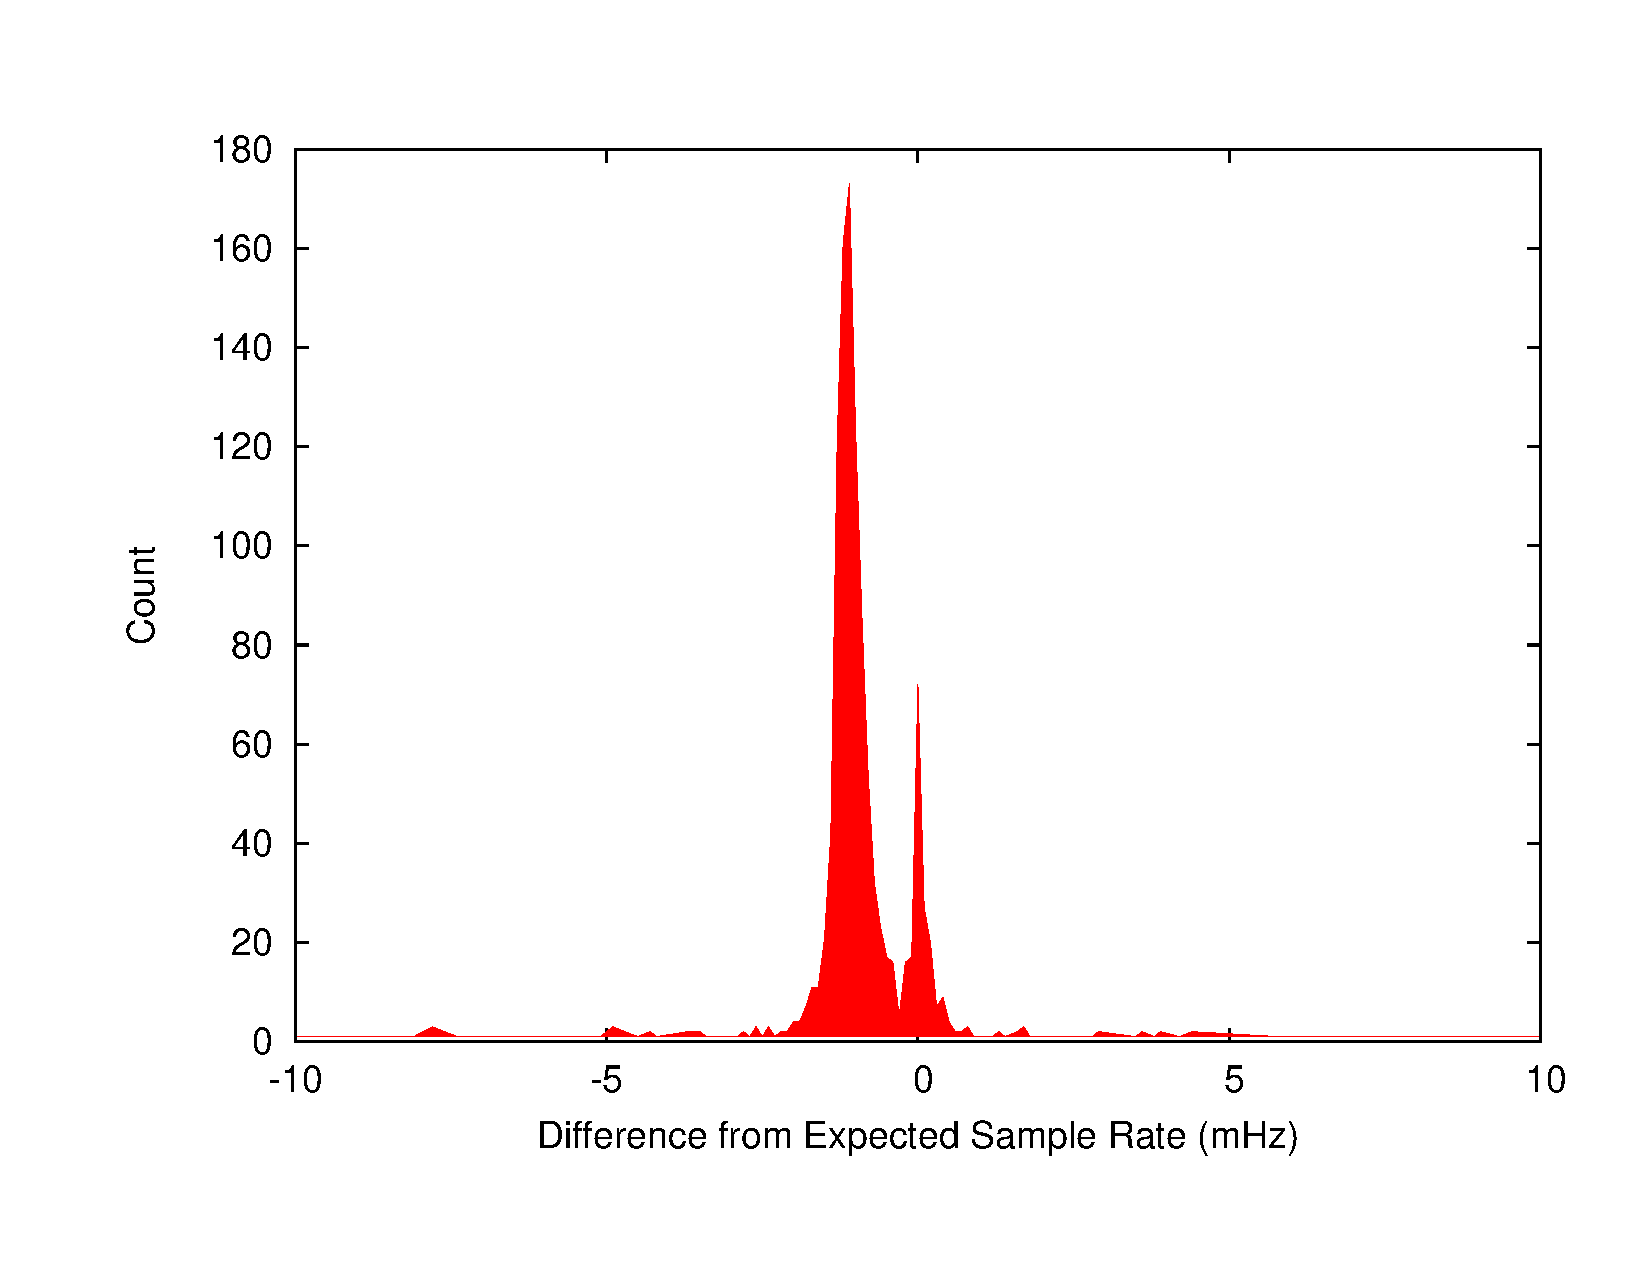
\includegraphics[width=\hsize]{./casestudy/figs/timing/SampleRates/SAMPLERATESHISTOGRAM.pdf}
%\end{center}
%\caption{\small{\bf Histogram of Output Sample Rate on Data Records}
%{\em As a first step in the data ground truthing we examined the apparent
%sample rate on each data record that emerged as an output of the time
%rectification process.  Data sampling was driven by an 50 parts-per-million
%oscillator on the interface board independent of the oscillator used for
%FTSP. What this figure shows is that on data records that we were able to
%time rectify the sample rates that emerge conform to the rates we would
%expect from the oscillator on board the interface board. \GWAnote{Not sure we
%need this and maybe it should be a CDF?}}}
%\label{fig-samplerates}
%\end{figure}

%\begin{figure}[t]
%\begin{center}
%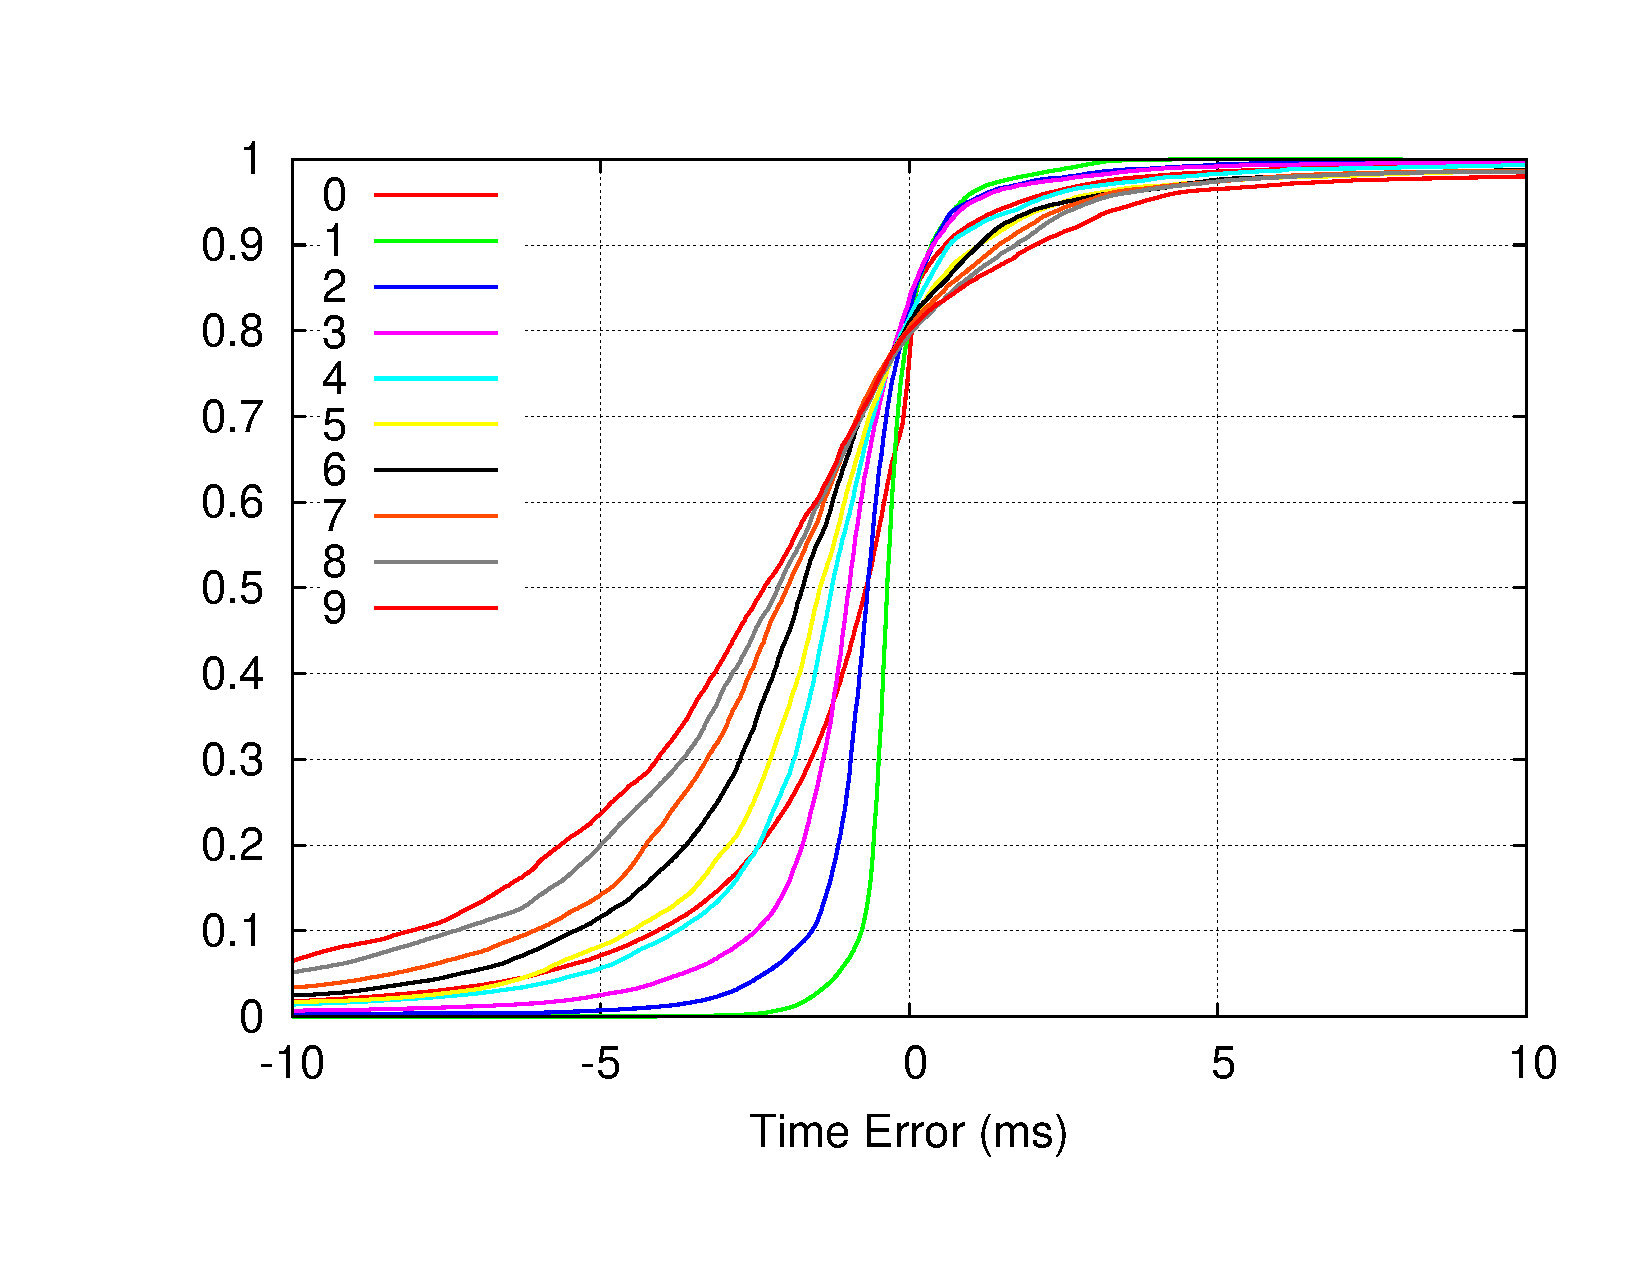
\includegraphics[width=\hsize]{./casestudy/figs/timing/TelosLabTiming/ABSOLUTEERROR.pdf}
%\end{center}
%\caption{\small{\bf Distribution of Bench Test FTSP Global Time Errors}
%{\em During the experiment described in Section~\ref{} we used periodic
%heartbeat messages to collect synchronous local time, global time pairs
%across the network.  This graph shows the distribution of the errors with
%respect to the ``true'' global time, that is the stamp recorded on the
%broadcast node when it sent the message.  FTSP performed well: FIXME\% of
%global timestamps reported by nodes within FIXME hops of the FTSP root had
%errors of less than FIXME ms. \GWAnote{This graph should probably show
%absolute values. I'm not sure its worth getting into why this shows a bias in
%one direction or the other...}}}
%\label{fig-absoluteerror}
%\end{figure}

%\begin{figure}[t]
%\begin{center}
%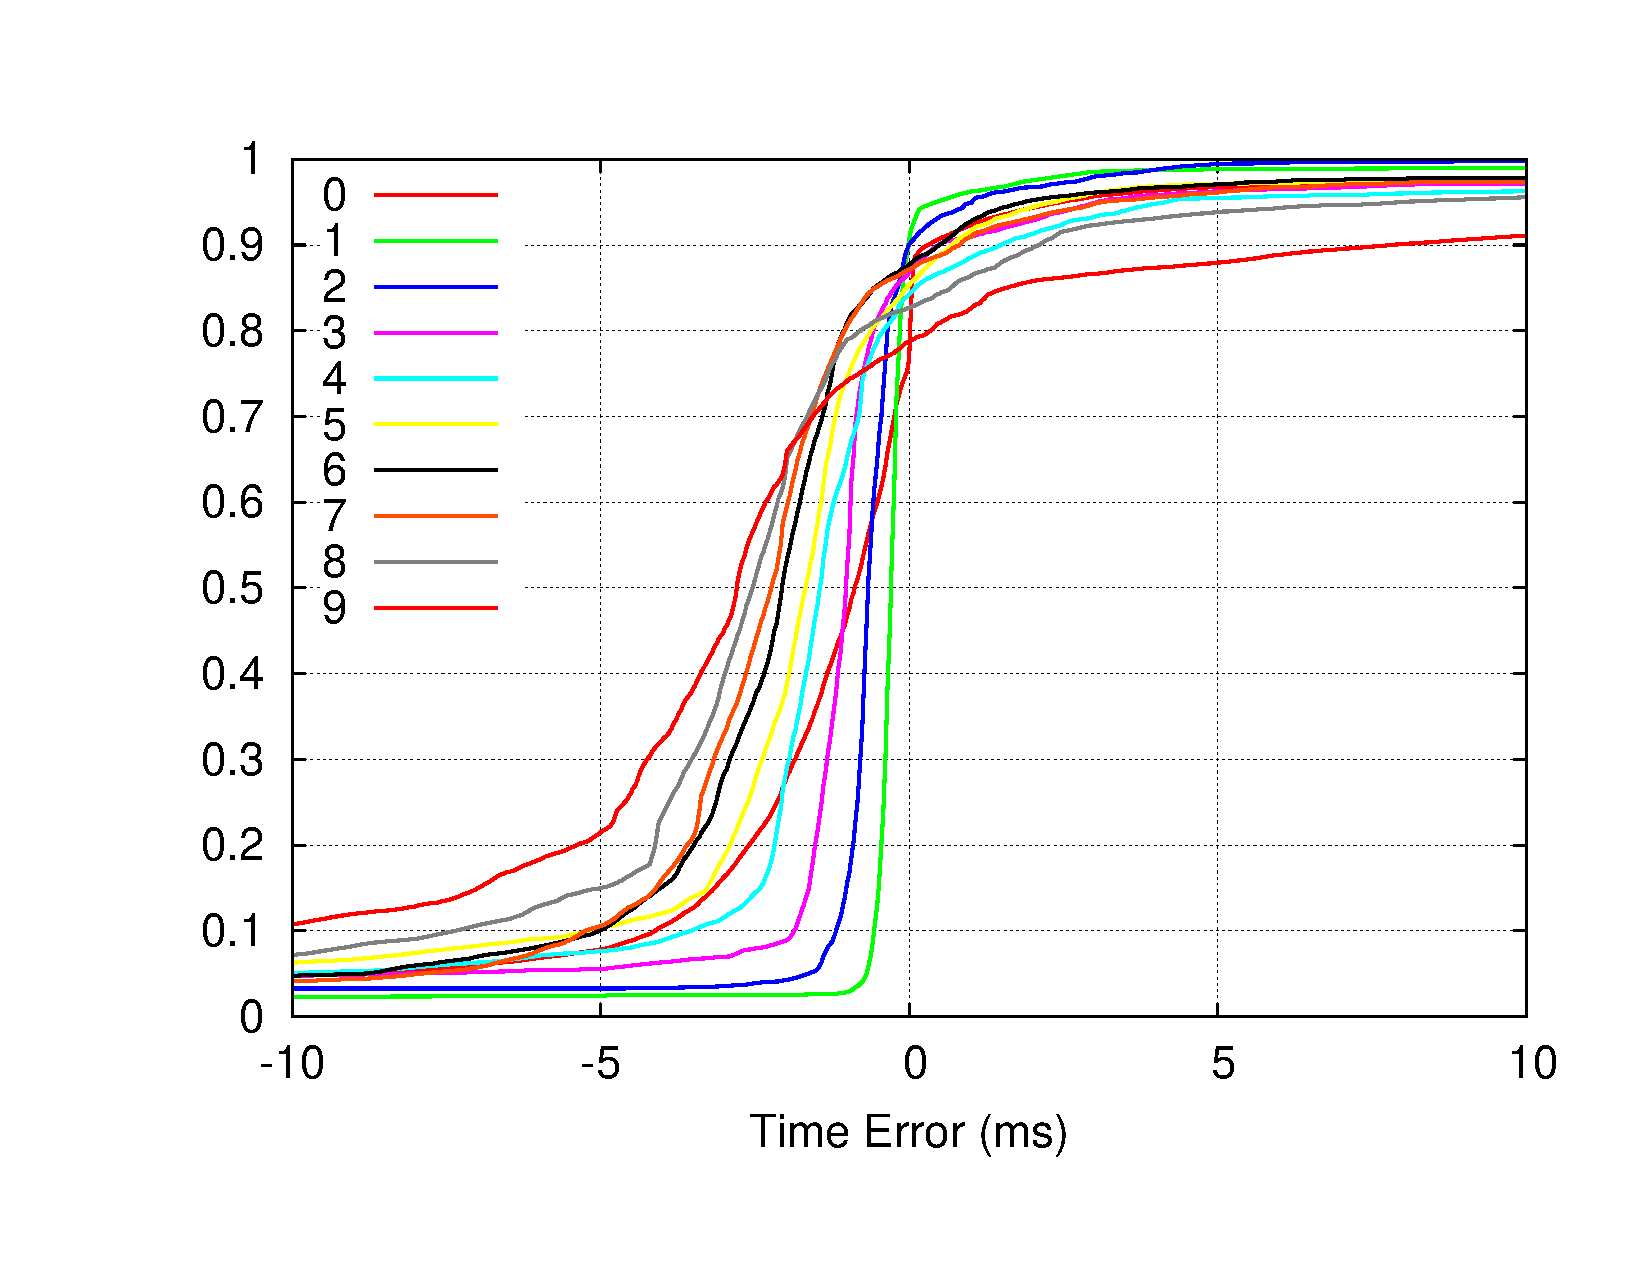
\includegraphics[width=\hsize]{./casestudy/figs/timing/TelosLabTiming/MAPPEDERROR.pdf}
%\end{center}
%\caption{\small{\bf Distribution of Bench Test Local to Global Time Mapping Error} 
%{\em For the experiment described in Section~\ref{} we simulated the time
%rectification process by using time data points collected in the status
%messages to map local time values onto known good global time values.  This
%graph shows the distribution of the result errors.  As the graph shows
%FIXME\% of local timestamps collected by nodes within FIXME hops of the FTSP
%root could be rectified to within FIXMEms of the true value. \GWAnote{See the
%note on the other figure like this.}}}
%\label{fig-mappederror}
%\end{figure}

%\begin{figure}[t]
%\begin{center}
%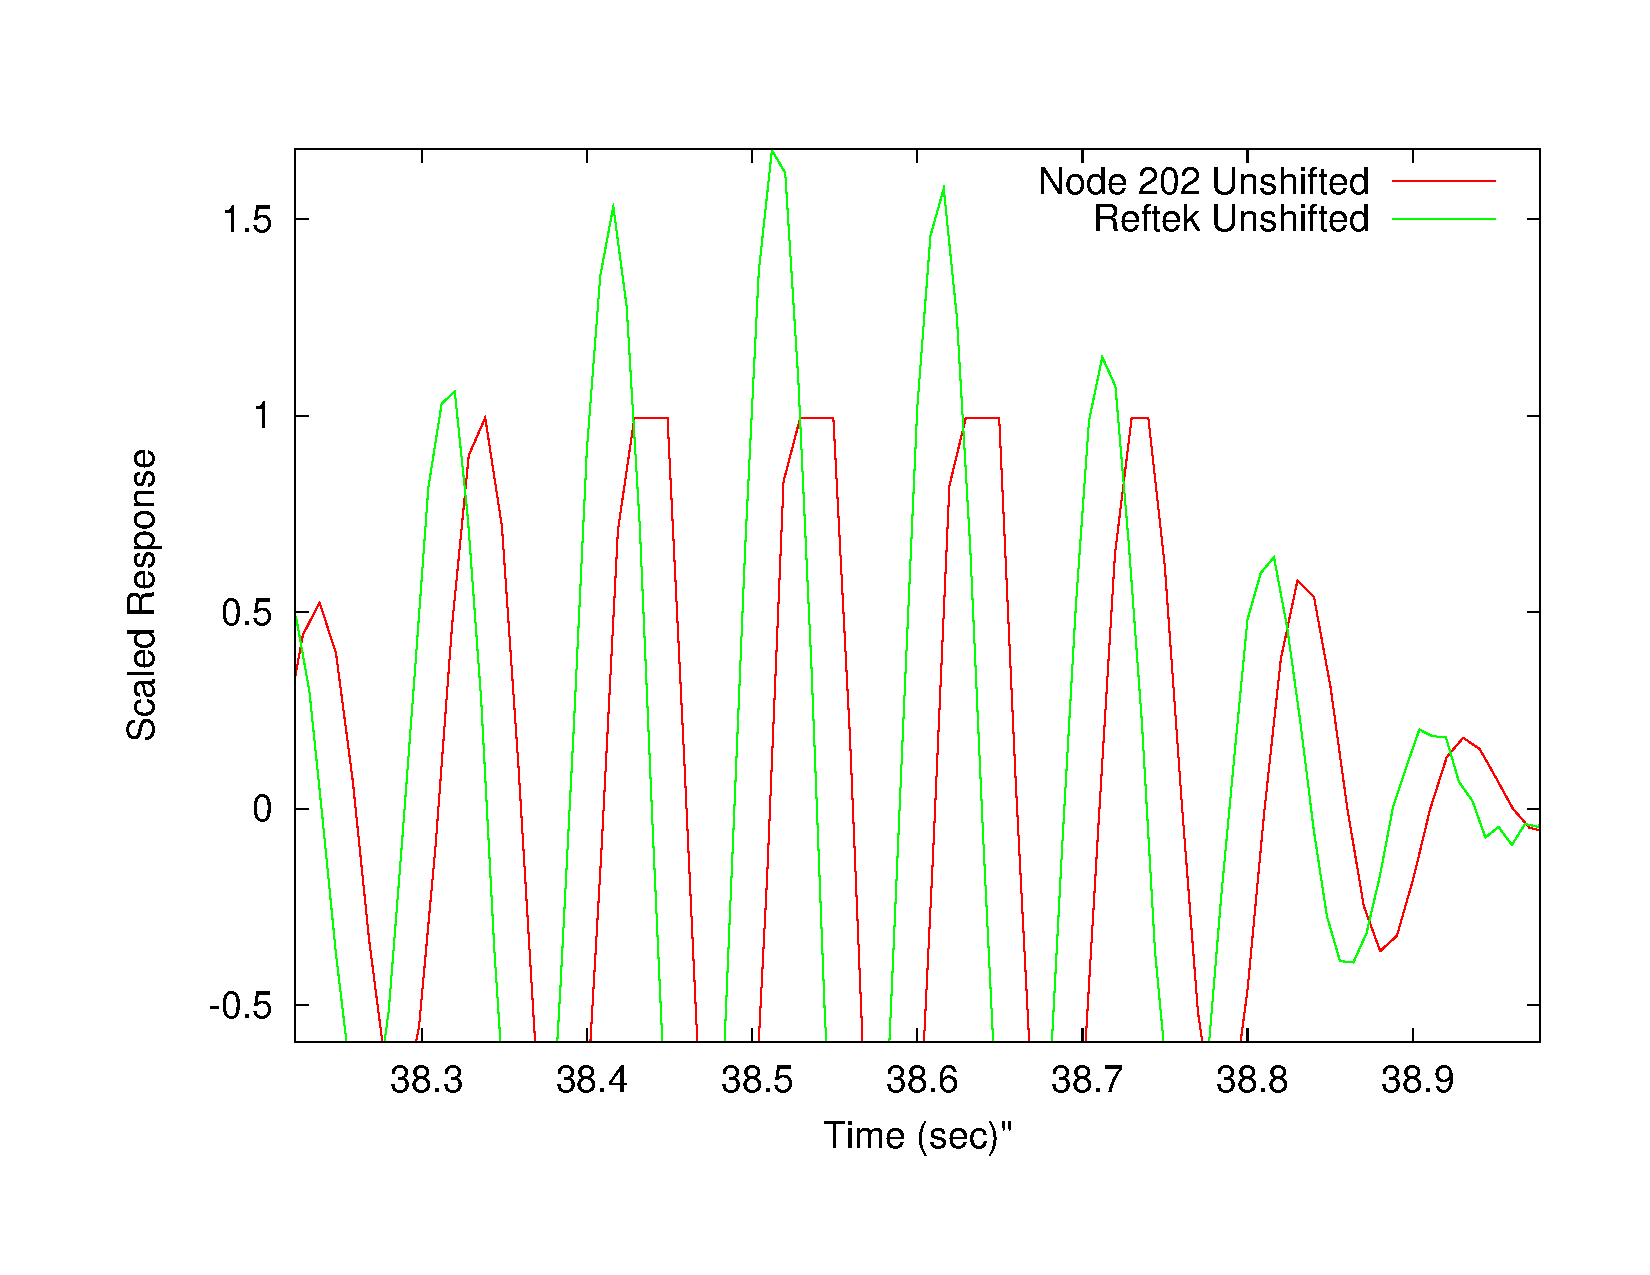
\includegraphics[width=\hsize]{./casestudy/figs/timing/FirstReftekComparison/COMPARISON-UNSHIFTED.pdf}
%\end{center}
%\caption{\small{\bf Reftek Side-by-side Test Signals Unshifted}
%{\em \GWAnote{I'm not sure we need to show this.  Or maybe we should, and
%talk about how we used this to discover the ``hidden'' 15ms delay?  Might be
%a better story than the shifted graph.}}}
%\label{fig-comparisonunshifted}
%\end{figure}

%\begin{figure}[t]
%\begin{center}
%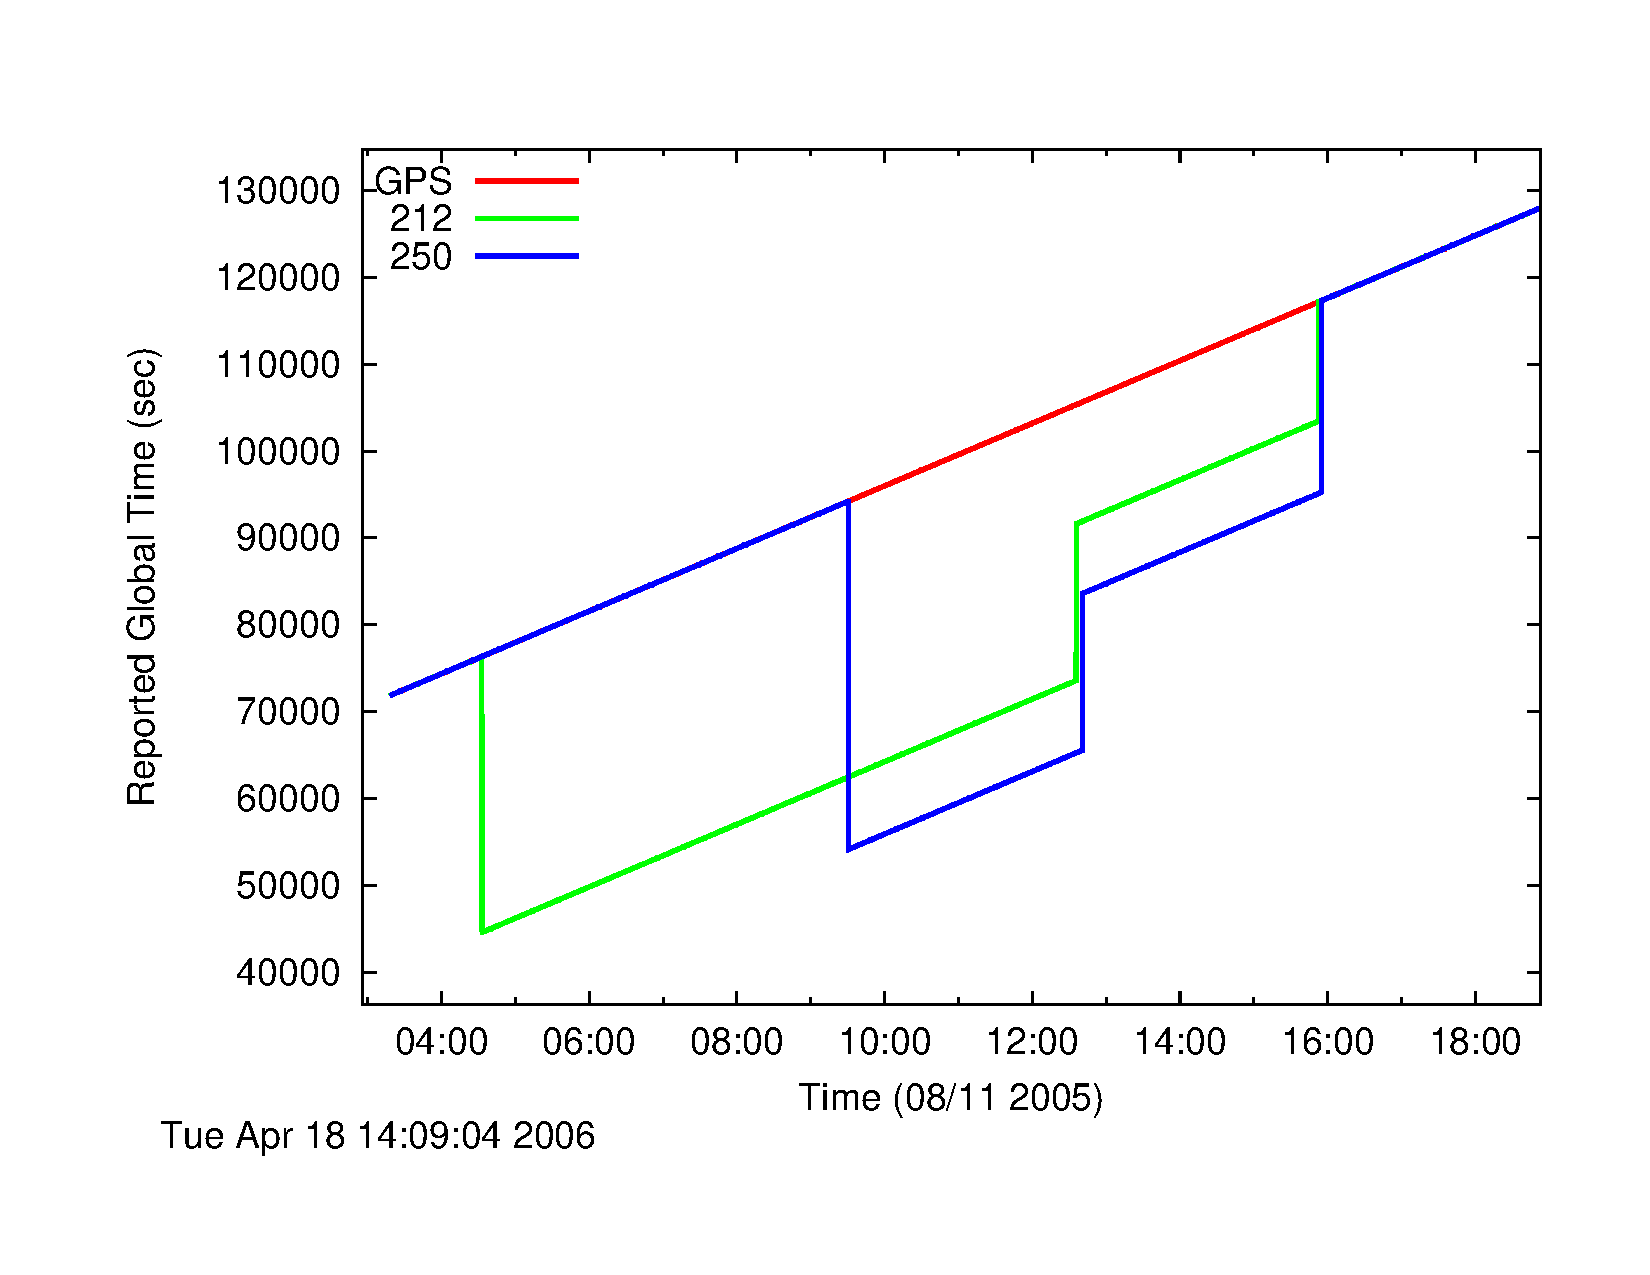
\includegraphics[width=\hsize]{./casestudy/figs/timing/GlobalTimeProblem/GlobalTimeProblem.pdf}
%\end{center}
%\caption{\small{\bf Example of FTSP Instability Observed During Field
%Deployment}
%{\em As describe in Section~\ref{timing-deploymentfailures} FTSP experienced
%periods of instability during our field experiment.  This graph shows an
%example of what we noticed in the field.  The global time value reported by
%two nodes and the GPS node is plotted against the time that the observatory
%laptop received the status message. At first all the lines are on top of each
%other.  However the graph shows that around 0400 GMT Node 212 began reporting
%a global time off by some 30,000 seconds, or over 8 hours. At around 0930 GMT
%Node 250 also began reporting an erroneous global time value. Although they
%both seem to make corrections at around 0100 hours they do not rejoin the GPS
%node until 1600 hours, producing 4.5 hours of global time downtime for Node
%250 and 9.5 for Node 212.  Although the heuristic filtering described in
%Section~\ref{timing-deploymentfailures} can identify and remove these
%timestamps no data collected by nodes during long outages such as this one
%can be correctly timestamped. Note that the absolute value of the global time
%value shown on the Y-axis is meaningless; global time values are mapped onto
%GMT time using techniques described in Section~\ref{section-timerectification}.}}
%\label{fig-globaltimeproblem}
%\end{figure}

%\begin{figure}[t]
%\begin{center}
%\includegraphics[width=\hsize]{./casestudy/figs/timing/MDW/rectification/rectify-STEP1.pdf}
%(a)
%\includegraphics[width=\hsize]{./casestudy/figs/timing/MDW/rectification/rectify-STEP2.pdf}
%(b)
%\end{center}
%\caption{\small{\bf Operation of the Heuristic Filter}
%{\em The two figures above show the operation of the heuristic filter. Figure
%(a) shows the raw $(localtime,globaltime)$ pairs collected from the node and
%shows that it experiences a period of FTSP instability.  Figure (b) shows
%that errant timestamps have been removed and a mapping between $localtime$
%and $globaltime$ created.}}
%\label{fig-rectificationprocess}
%\end{figure}

%\begin{figure}[t]
%\begin{center}
%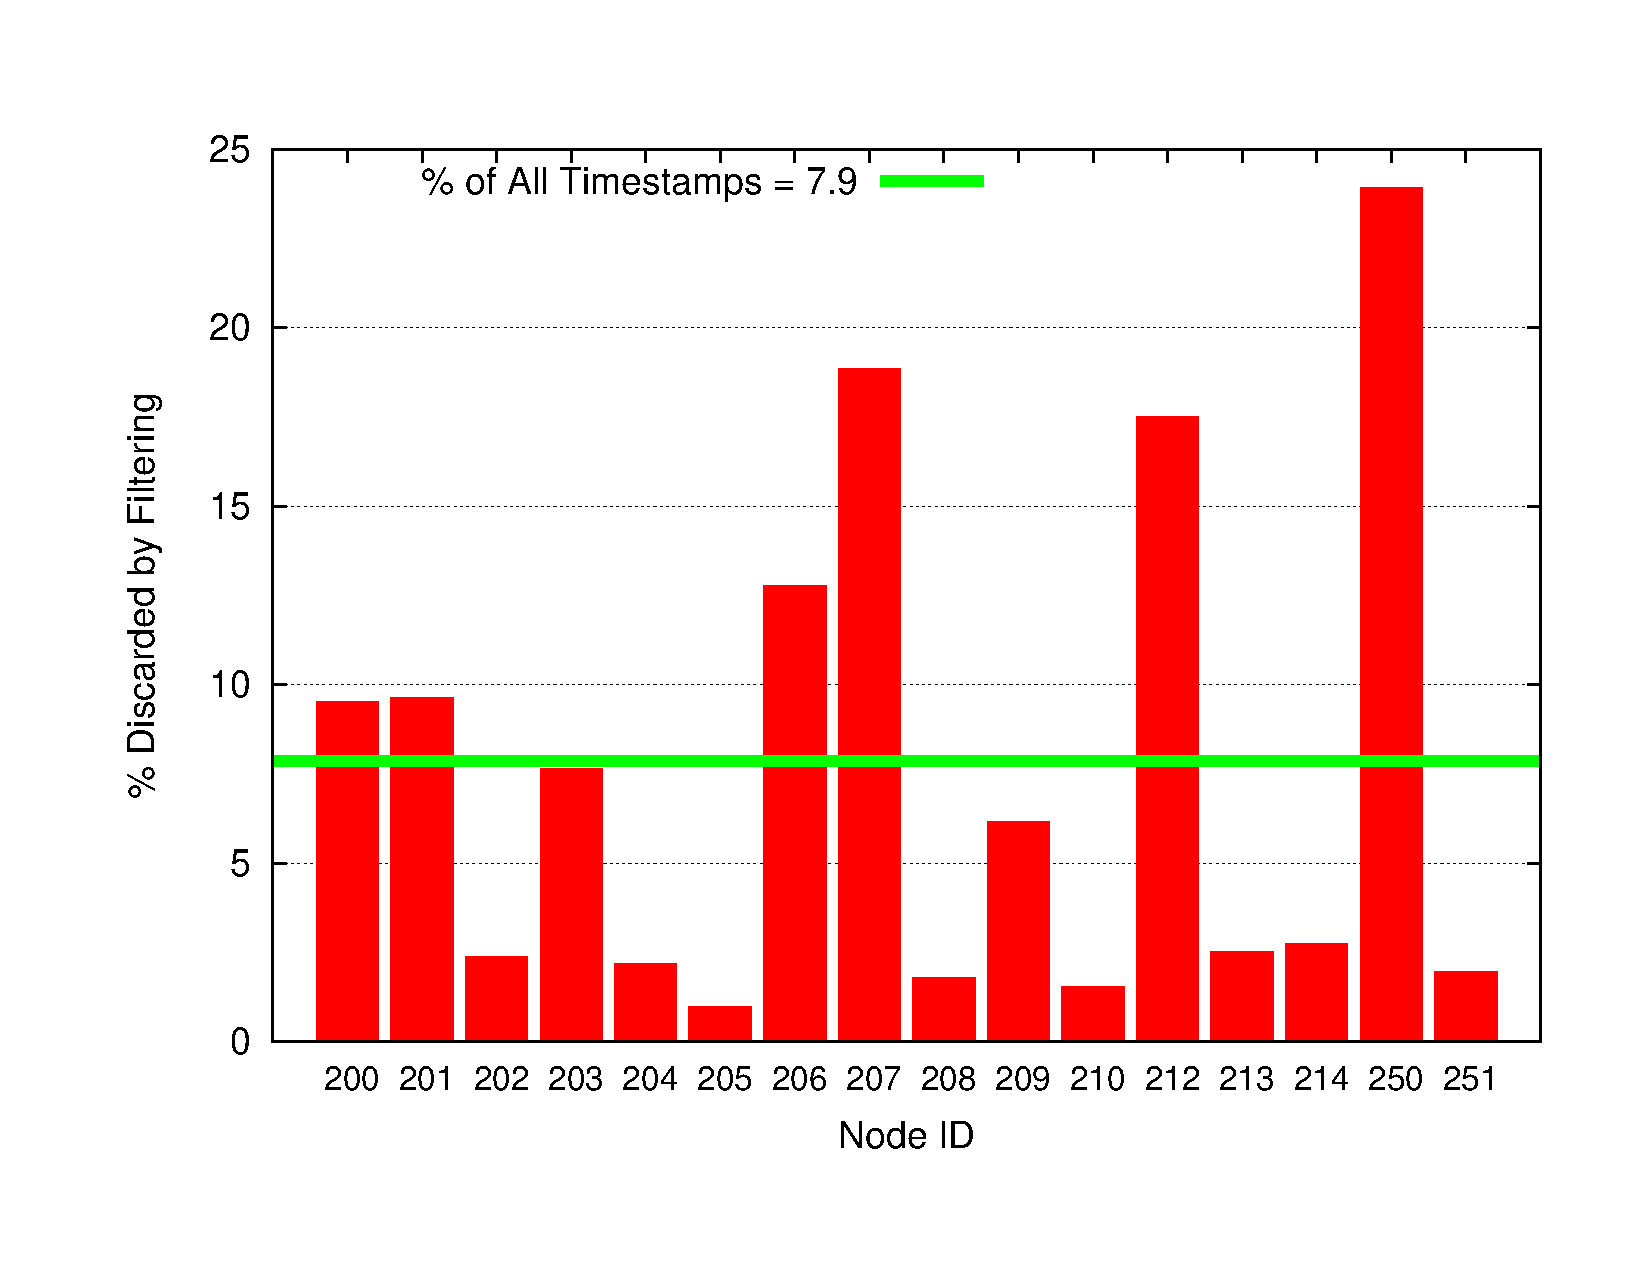
\includegraphics[width=\hsize]{./casestudy/figs/timing/FTSPUpDown/FTSPDOWN.pdf}
%\end{center}
%\caption{\small{\bf Percentage of timestamps discarded by filtering.}
%{\em Overall, the filter rejected \XXXnote{7.9\% ???} of the time 
%stamps reported by sensor nodes. However, certain nodes, such as
%node~250, had an unusually large number of FTSP failures.}}
%\label{fig-ftspdown}
%\end{figure}

